% TODO
% Show how tensor product + swap gates can generate all needed matrices
% Explain Schrodinger equation for QA
% Why does Grover's algorithm have that many steps
% 4.1 replace with PDF circuit
% why ain't assoc workin

\documentclass[11pt]{report}
\usepackage{graphicx}
\usepackage[font=footnotesize, labelfont={sf,bf}, margin=1cm]{caption}
\usepackage{mathtools}
\usepackage{wrapfig}
\usepackage[letterpaper, portrait, margin=1in]{geometry}
\usepackage{framed}
\usepackage{listings}
\usepackage{color}
\usepackage{float}


\usepackage[mathletters]{ucs}
\usepackage[utf8x]{inputenc}

\usepackage{enumerate}
\usepackage[titletoc,toc,title]{appendix}
\usepackage{amsfonts}
\usepackage{amssymb}
\usepackage{tikz}
\usepackage[section]{placeins}
\usepackage{braket}
\newcommand{\?}{\stackrel{?}{=}}
\definecolor{mauve}{rgb}{0.58,0,0.82}
\lstset{frame=tb,
  language=Lisp,
  aboveskip=3mm,
  belowskip=3mm,
  showstringspaces=false,
  columns=flexible,
  basicstyle={\small\ttfamily},
  numbers=none,
  numberstyle=\tiny\color{gray},
  keywordstyle=\color{blue},
  commentstyle=\color{cyan},
  stringstyle=\color{mauve},
  breaklines=true,
  breakatwhitespace=true,
  tabsize=3
}

\usepackage{import}
%\newcommand{\braket}[1]{\ensuremath{\left | #1 \right \rangle}}
\newcommand{\qcol}[2]{\ensuremath{\begin{pmatrix} #1 \\ #2 \end{pmatrix}}}

%Gummi|065|=)
\title{\textbf{Theory and Applications of Quantum Computing}}
\author{William Bernoudy\\ \\
		Mentor: Richard Hoshino}
\date{\today}
\begin{document}
\maketitle

\setcounter{tocdepth}{1}
\tableofcontents

\chapter{Motivation for Quantum Computing}

Moore’s law states that the number of transistors that can be manufactured at a given cost will double approximately every two years \cite{moo65}. As the transistor count on a microchip is proportional to computing power, the law implies that the computational power available for a given amount of money doubles every two years. The entire progression of modern technology is essentially reliant upon Moore's law and the seemingly untethered growth of computing power. Companies are able to release significantly more powerful devices each year that are smaller and more power efficient. Every year new software is released that takes advantage of the increase, allowing users to use more powerful programs with increased capability, with less waiting time for the computing processes to be completed. Moore's law has held true since the dawn of the microchip until at least very recently. However, there are physical limits to the law that prevent it from continuing indefinitely. One of the most obvious is the size of transistors. Currently, 10 nm transistors are being put into production by Intel \cite{Sim16}. However, transistors any smaller than 7 nm will start to experience the effects of quantum tunneling, where electrons flowing through one part of the transistor will ``tunnel" through the silicon barrier to other parts, making the production of these transistors significantly more difficult \cite{Kha15}. Physical restrictions such as this will make the continuation of the law increasingly infeasible. 

However, the end of Moore’s law does not mean the end of the progression of computation. Quantum computing offers an alternative to computing on silicon chips. While quantum computers are superior to classical (e.g. transistor-based) computers only for a limited class of problems, these problems have wide-reaching applications in many fields such as machine learning, protein folding, search algorithms, and optimization problems. Many of these problems are able to be completed in exponentially shorter periods of time on quantum computers \cite{apps14}. Though quantum computers will never replace classical computers, their possible applications include exciting and important future developments.

I chose to study quantum computing mainly because I believe it will play a crucial role in the development of certain technologies that will benefit many people in the same way conventional computing has. For example, understanding protein folding allows researchers to develop better drugs to prevent and cure diseases such as HIV/AIDS and cancer, and quantum computing may allow us to achieve more on this front than conventional computers ever will \cite{foldit}. I also appreciate the way that quantum computing attempts to repurpose some of the strangest observed phenomena central to the fundamental nature of the universe to perform certain types of computations faster. 

To accomplish this goal, I took classes such as Linear Algebra and Complex Analysis which helped me form an understanding and familiarity of the underlying concepts behind quantum computing. I then used self-study of quantum computing textbooks, research articles and blog posts by experts in the field to learn the basics of quantum computing. I also used several final projects in various classes as opportunities to expand my understanding by implementing common quantum algorithms. Finally, I interned at D-Wave Systems, currently the only company in the world producing quantum computers. During the internship, I worked with an algorithms researcher\footnote{Andrew King, aking@dwavesys.com.} to find the best way to run a certain type of problem on their computers.

\section{Outline of Keystone}
In chapter 2, I outline the developments in physics that led to the modern understanding of the quantum world, explain how conventional computing can be modeled using linear algebra, explain the basics of quantum computing, and then touch on the different types of quantum computation.

In chapter 3, I explain how it is possible to simulate a gate-based quantum computer on a conventional computer as well as describe more precisely what a quantum computer does using a mathematical construct, and then introduce the simulator I wrote.

In chapter 4, I discuss Grover's algorithm and its applications, describe how it works, and explain my implementation of it using my quantum computer simulator.

In chapter 5, I describe an associative memory algorithm and show my implementation of it on the same simulator.

In chapter 6, I show how to recursively construct a quantum circuit which implements the quantum Fourier transform.

In chapter 7, I explain quantum annealing and its application to solving Ising problems, compare it to simulated annealing, and discuss the difficulties with programming and using D-Wave's actual quantum annealing machine.

Finally, in chapter 8, I conclude my Keystone, discuss some of the problems quantum computing faces and what I aim to do in the future.

\chapter{Introduction to Quantum Computing}

\section{Quantum Mechanics}
At the dawn of the twentieth century, Max Planck made the amazing discovery that the energy level of an electromagnetic wave, i.e. light, is quantized \cite{meh01}. Instead of being continuous, as previously thought, Planck discovered that there is a lower limit on level of energy that an electromagnetic wave can have, and that the energy must always be a multiple of this lower bound, called Planck's constant. In other words, the energy of an electromagnetic wave is divided up into discrete ``quanta," or packets of energy. The word ``quantum" is derived from this discovery.

Einstein expanded on Planck’s findings and found that light can be modelled not only as a wave, as was the case in physics previously, but also as a particle \cite{ein05}. The corresponding particle for light is called a photon. This led to the discovery of the wave-particle duality of nature, one of the fundamental principles of quantum mechanics. The wave-particle duality states that every particle or packet of energy has the properties of both waves and particles. Quantum mechanics was developed as a result of this discovery. Scientists found that quantum mechanics did an extraordinary job of explaining certain phenomena on tiny scales that classical physics could not explain. For example, take the ``orbit" of an electron around the nucleus of an atom. According to classical physics, the orbit would decay and the ``orbit" could not be stable \cite{smi15}.

In 1926, Erwin Schrödinger published a paper outlining a new equation, called ``Schrödinger’s wave equation," that modelled quantum physics \cite{schr26}. In the quantum understanding, all properties of a physical system are modeled by a wave function which describes the different probabilities of the system being in any of its possible configurations. This means that before the system is measured by an observer, the system exists simultaneously in some amount of all of its possible states. When they are measured, i.e. when the wave function collapses, a system state is chosen seemingly at random according to the probability distribution. Schrödinger's wave equation models the evolution of the wave function of a physical system over time. It does not predict what the actual values will be, but instead gives a spread of the probabilities for the different values one might get when the system is measured.

Schrödinger's wave equation results in some interesting properties of matter. One of these, which allows for a basis for quantum computation, is called quantum superposition. Because of a certain attribute of the solutions to the wave equation (their linearity), matter can exist in an overlap of many different states. For example, let's say we have some electrons traveling in a circuit of conductive material. In the classical understanding, the electrons must be traveling in one of the two possible directions. In the quantum mechanical understanding, as long as we do not disturb the circuit in any way (which is equivalent to observation or the wave collapsing), the electrons can actually flow both ways at once. We could then use Schrödinger's wave equation to determine the likelihood of the electrons flowing in one direction or another once we measure the system.

\section{Classical Computation}
Classical computation usually consists of two components: memory and a processor. In the memory, binary information is stored in the form of bits. A bit is a single piece of binary data, meaning it is either a zero or a one; the information that we desire to process must thus be encoded in a sequence of zeros and ones. The processor is simply a device that performs different operations on the bits in the memory.

At any given point in time, we can talk about the system state of the processor. This essentially consists of the value of the bits in the memory. For a processor that runs $n$ bits, the memory must be in one of $2^n$ possible states. For example, if we have a processor that uses a 2-bit architecture, the memory has 2 bits. This means that at any point during our processing, we could examine the memory and see that it will be in one of $2^2=4$ possible states:
$$00$$
$$01$$
$$10$$
$$11$$

Another way of representing the states of a classical computer is with vectors. Though unnecessary to understand classical computation, vectors will help tremendously when trying to understand quantum computation. Instead of using a zero or a one to represent the state of one bit, we can use a two dimensional vector:
$$\left | 0 \right \rangle=\begin{pmatrix}1\\ 0\end{pmatrix} \quad \left | 1 \right \rangle=\begin{pmatrix}0\\ 1\end{pmatrix}$$
             
These are the two binary states of a single bit. We use two dimensional vectors so that the 0 and 1 states are linearly independent, which will allow us to combine the states without mixing when we model quantum computers. The $\left | 0 \right \rangle$ notation is simply used to indicate that in this case, we are talking about the vector that corresponds to the value of 0 in our system. 

For computers with more than one bit, we are actually dealing with vectors in higher dimensional space. If we have a processor with $n$ bits, then the vectors that correspond to the different states of the machine will have $2^n$ dimensions. We can see this holds true for the single bit processor, because it has $2^1=2$ dimensions. For a classical computer, the number of dimensions created by its bits is equal to the total number of possible states of the computer. Each state of the computer corresponds to a vector pointing directly in one of the $2^n$ dimensions with a magnitude of 1.

To calculate a system's state vector from the states of its bits, we can use the \textit{tensor product} of all the states of the individual bits. The tensor product for matrices, also called the Kronecker product and denoted as $\otimes$, is a matrix operation defined for any two matrices that produces a third matrix in a way that generalizes the outer product of two vectors. For an $m$ by $n$ matrix $\mathbf{A}$ and a $p$ by $q$ matrix $\mathbf{B}$, the tensor product of $\mathbf{A}$ and $\mathbf{B}$ is an $mp$ by $nq$ matrix is
$$\mathbf{A}\otimes\mathbf{B} = \begin{bmatrix} a_{11} \mathbf{B} & \cdots & a_{1n}\mathbf{B} \\ \vdots & \ddots & \vdots \\ a_{m1} \mathbf{B} & \cdots & a_{mn} \mathbf{B} \end{bmatrix}$$

where $a_{ij}\mathbf{B}$ is expanded wherever it has been placed in the resulting matrix. The following example illustrates the tensor product of two $2\times2$ matrices:

$$
  \begin{bmatrix}
    1 & 2 \\
    3 & 4 \\
  \end{bmatrix}
\otimes
  \begin{bmatrix}
    0 & 5 \\
    6 & 7 \\
  \end{bmatrix}
=
  \begin{bmatrix}
    1\cdot 0 & 1\cdot 5 & 2\cdot 0 & 2\cdot 5 \\
    1\cdot 6 & 1\cdot 7 & 2\cdot 6 & 2\cdot 7 \\
    3\cdot 0 & 3\cdot 5 & 4\cdot 0 & 4\cdot 5 \\
    3\cdot 6 & 3\cdot 7 & 4\cdot 6 & 4\cdot 7 \\
  \end{bmatrix}
=
  \begin{bmatrix}
    0 & 5 & 0 & 10 \\
    6 & 7 & 12 & 14 \\
    0 & 15 & 0 & 20 \\
    18 & 21 & 24 & 28
  \end{bmatrix}.
$$

Armed with the tensor product, we can compute the system state vector from the states of all its bits. For a system state $S$ and its bits $b_1, b_2, \ldots, b_n$, we have

$$\left | S \right \rangle = \left | b_1 \right \rangle \otimes \left | b_2 \right \rangle \otimes \cdots \otimes \left | b_n \right \rangle$$

This works out to a simple pattern. First, let $k$ equal the bit string $b_1b_2\ldots b_n$ interpreted as a base 2 number. Then $S$ will be equal to a vector consisting of all zeros with a single 1 in the $(k+1)$th position. For example, take a 3-bit computer in the state 011. We can calculate $S$ as follows:

$$\left | S \right \rangle = \left | 0 \right \rangle \otimes \left | 1 \right \rangle \otimes \left | 1 \right \rangle = \qcol{1}{0} \otimes \qcol{0}{1} \otimes \qcol{0}{1} = \begin{pmatrix}0\\0\\0\\1\\0\\0\\0\\0\end{pmatrix}$$

Note that $011_2 = 3$, and that the 1 in the resulting vector is in position 3+1=4.

For any classical computer with a selection of bits, each bit can only be in two possible states, and so the computer must always be in one of $2^n$ possible states. This means that its state vector will have $2^n$ dimensions, and will always be pointing directly in just one of those dimensions. Any computation that we carry out on that state will always result in the vector switching to pointing directly in a new dimension with a magnitude of 1. However, this is just one way of representing information; quantum computing offers a radically different approach where the state vector is not limited to just one state at a time.

\section{Quantum Computing}
A quantum computer is a computer that takes advantage of quantum phenomena. Specifically, it is a computer based on \textit{qubits} instead of bits. Qubits are pieces of information that can have states and interact in ways not possible with a classical understanding. For example, unlike a classical bit, a qubit can be in a superposition of multiple states at once.

Let’s say we have one qubit called $\psi$. Its vector is given by:
$$ \left | \psi \right \rangle=\alpha _{0}\left | 0 \right \rangle+\alpha _{1}\left | 1 \right \rangle=\begin{pmatrix}\alpha_{0}\\ \alpha_{1}\end{pmatrix}$$
where $\alpha _{0}$ and $\alpha_{1}$ are complex numbers satisfying the constraint 
$$ \left | \alpha_{0} \right |^{2} + \left | \alpha_{1} \right |^{2}=1$$
This means that the  values have an infinite number of possibilities. Unlike a classical bit, for which the vector could only consist of all zeroes and one ``1," there are an infinite number of directions $\psi$ can be pointing. This is a mathematical way of saying that $\psi$ is not really in either the $\left | 0 \right \rangle$ state or the $\left | 1 \right \rangle$ state, but in a superposition of both. It exists as some amount of both at the same time.

The $\alpha$ values, also called the amplitudes of their corresponding states, are often written as
$$\ket{\psi} = ae^{i\theta}\ket{0} + be^{i\phi}\ket{1}$$

where $a$, $b$, $\theta$ and $\phi$ are all real numbers. Because we have the same constraint as before, we also have that
$$1 = |ae^{i\theta}|^2 + |be^{i\phi}|^2 = |a(\cos{\theta}+i\sin{\theta})|^2 + |b(\cos{\phi}+i\sin{\phi})|^2$$
$$1 = a^2(\cos^2{\theta} + \sin^2{\theta}) + b^2(\cos^2{\phi} + \sin^2{\phi})$$
$$1 = a^2 + b^2$$ 

Because $a$ and $b$ also must satisfy this normalization constraint, we can represent them both with just a single value on the interval [0,1]. Thus we can represent a single qubit with just three real values: $\theta$, $\phi$, and $a$, where $b = \sqrt{1 - a^2}$. The Bloch sphere visualizes this representation. When the qubit is pointed directly upward (the positive z-axis), it has a value of $\ket{0}$. When it is pointed directly downwards (the negative z-axis), it has a value of $\ket{1}$. Thus the z-axis corresponds to the normalized $a$ and $b$ value (note that while $\ket{0}$ and $\ket{1}$ are shown on the same axis, they are still linearly independent basis vectors).  Unlike the bit, we can see that there are now two axes of rotation afforded to the qubit that were not present before. However, the current state of the qubit in the Bloch sphere remains on the surface of the sphere. We can see in this example that it is pointed more closely upwards, towards the $\ket{0}$ vector, than it is downwards. This means that if we were to observe this qubit, it is more likely that it would collapse to the $\ket{0}$ state. If the qubit were pointed more towards the bottom of the sphere at the $\ket{1}$ vector, it would be more likely that we would collapse to the $\ket{1}$ state.

\begin{figure}[!h]
    \centering
    \def\svgwidth{2in}
    \import{resources/pdfs/}{Bloch_Sphere.pdf_tex}
    \caption{The Bloch sphere}
    \label{fig:awesome_image}
\end{figure}

The variability of qubits is furthered amplified when adding more qubits. Like the classical computer, the possible states for an $n$-qubit quantum computer exist in a $2^{n}$ dimensional space. However, this time, the vector which represents the state of the qubits does not have to be pointing in only one of the dimensions --- it can exist in all of them (i.e. it can be in a superposition of all of them). For example, if we have a 3-qubit system, then the general state of the qubits, is given by:

$$ \left | \mathbf{\Psi} \right \rangle=\alpha _{000}\left | 000 \right \rangle+\alpha _{100}\left | 100 \right \rangle+\alpha _{010}\left | 010 \right \rangle+\alpha _{110}\left | 110 \right 
                \rangle+\alpha _{001}\left | 001 \right \rangle+\alpha _{101}\left | 101 \right \rangle+\alpha _{011}\left | 011 \right \rangle+\alpha _{111}\left | 111 
                \right \rangle$$
                
$$\left | \mathbf{\Psi} \right \rangle=\begin{pmatrix}\alpha_{000}\\\alpha _{100}\\\alpha_{010}\\\alpha_{110}\\\alpha_{001}\\\alpha_{101}\\\alpha_{011}\\\alpha_{111}\end{pmatrix}$$

	Thus, at any point in the computation, the state of the qubits, $\mathbf{\Psi}$, can be described with a vector of length $2^{n}$. When we measure the system, it disturbs the ``quantum-ness" of the qubits, causing the wave function to collapse and to pick one value. The probability of the system collapsing into a certain state is given by the square of the magnitude of the $\alpha$ value corresponding to that state.

\section{The Gate Model of Quantum Computing}
To qualify as a quantum computer, a device or model must simply be able to do computation that takes advantage of quantum effects. This means that there are many approaches in the field to understanding quantum computing as well as distinct approaches to physical realizations. In this Keystone, I will discuss the two most common models: the gate model and quantum annealing. They have many similarities, and perhaps most importantly, the concept of representing the system state with a complex vector of length $2^n$ is common to both. 

The gate model of quantum computing (also called a universal quantum computer or a Quantum Turing machine) describes a model where discrete operations applied to the system predictably produce a new system state. In this sense, it is similar to way that we think about classical computing, where the system state exists in memory and then is passed into the processor, which then predictably modifies the system state and the outcome is loaded back into the memory. The famous quantum algorithms, such as Grover's algorithm and Shor's algorithm, are all described using the gate based model. It is also called a universal quantum computer because it is able to run any quantum algorithm with a polynomial overhead. However, researchers have struggled to make a device that is able to perform gate based algorithms in any meaningful way.

In the next chapter, I will explain how the gate-based model provides easy ways of simulating a universal quantum computer.

\chapter{Simulating a Gate-Based Quantum Computer}

Because the state of the computer can be represented with a single vector, an easy way to simulate quantum computation is to simply keep track of this vector. At the end of our computation, we can examine the vector to see which state the system is most likely to collapse into, and thus check to see if our computation worked.

To create a system of $n$ qubits, we simply make a vector length $2^{n}$ of all zeros. Then, just as with the classical computer, depending on what we want the initial values of qubits to be we make one of the zeros in the vector a 1. The position of the 1 corresponds to the decimal form of the binary representation of the bits, e.g. if we want to start with $\left | 100 \right \rangle$ as the initial state, then we would change the zero in position 5 of the vector to a 1.

Just like classical computation, quantum computation is done by causing the qubits to react in certain ways through ``quantum gates." In the same vein as the state of the computer, gates can conveniently represented as matrices. We can multiply the state of the system by a matrix corresponding to a gate to ``simulate" the gate, as the resulting vector will be representative of the system after it has gone through the gate \cite{spector04}.

For classical compuatation, where the state of the system must be vector consisting of all zeros and one ``1" (because it can only be in one state at once), the only valid matrices, meaning those that correspond to physically possible gates, are ones that always produce a valid system after the multiplication. If a matrix in classical computation produces anything but a vector of all zeros and one ``1", then we know it's invalid. However, quantum gates do not have this restriction. This means that matrices that produce vectors with lots of different values are perfectly fine; this actually just represents a superposition of different system states. In fact, the only restriction on quantum gates is that they are reversible and that their matrix form is a \textit{Hermitian} matrix. This means that if a quantum gate has the corresponding matrix operator $\mathbf{O}$, it is only a valid gate if $\mathbf{O}\mathbf{O}^* = \mathbf{O}^*\mathbf{O} = I$, where $\mathbf{O}^*$ denotes the adjoint of $\mathbf{O}$ (i.e. $(\mathbf{O}^*)_{ij} = \overline{\mathbf{O}_{ji}}$, with $\overline{\mathbf{O}_{ji}}$ being the complex conjugate of $\mathbf{O}_{ji}$).

The superposition principle of quantum mechanics states that any two valid quantum states can be combined linearly to create another valid state. This is a result of the fact that the Schrödinger equation is a linear equation, so any of its solutions (which are wave functions, or in our case, system states of the qubits in our quantum computer) can also be combined linearly. This principle is the reason for why we can model any gate as a matrix, as a gate is simply a linear combination of the previous amplitudes of each possible state of the system. Similarly, matrix multiplication on a vector defines a linear transformation.

Most quantum gates only act on 1, 2 or 3 qubits. Some common examples include the three Pauli matrices

\begin{table}[h!]
\centering
\begin{tabular}{ c c c }
  $\begin{pmatrix}
0 & 1 \\
1 & 0 \\
\end{pmatrix}$ & $\begin{pmatrix}
0 & -i \\
-i & 0 \\
\end{pmatrix}$ & $\begin{pmatrix}
1 & 0 \\
0 & -1 \\
\end{pmatrix}$ \\
  Pauli-x & Pauli-y & Pauli-z \\
\end{tabular}
\end{table}

The Pauli-x matrix, also called a NOT gate, ``flips" the value of a single qubit, taking $\ket{0}$ to $\ket{1}$ and vice versa. It is equivalent to rotating the qubit state $\pi$ radians around the x-axis on the Bloch sphere. The Pauli-y and z matrices also rotate the qubit state $\pi$ radians on the Bloch sphere around the y and z axes respectively.

Other common examples include the Hadamard, CNOT, SWAP and the Toffoli gates

\begin{table}[h!]
\centering
\begin{tabular}{ c c c c }
$\frac{1}{\sqrt{2}}\begin{pmatrix}
1 & 1 \\
1 & -1 \\
\end{pmatrix}$ &
$\begin{pmatrix}
1 & 0 & 0 & 0 \\
0 & 1 & 0 & 0 \\
0 & 0 & 0 & 1 \\
0 & 0 & 1 & 0 \\
\end{pmatrix}$ & 
$\begin{pmatrix}
1 & 0 & 0 & 0 \\
0 & 0 & 1 & 0 \\
0 & 1 & 0 & 0 \\
0 & 0 & 0 & 1 \\
\end{pmatrix}$ & 
$\begin{pmatrix}
1 & 0 & 0 & 0 & 0 & 0 & 0 & 0 \\
0 & 1 & 0 & 0 & 0 & 0 & 0 & 0 \\
0 & 0 & 1 & 0 & 0 & 0 & 0 & 0 \\
0 & 0 & 0 & 1 & 0 & 0 & 0 & 0 \\
0 & 0 & 0 & 0 & 1 & 0 & 0 & 0 \\
0 & 0 & 0 & 0 & 0 & 1 & 0 & 0 \\
0 & 0 & 0 & 0 & 0 & 0 & 0 & 1 \\
0 & 0 & 0 & 0 & 0 & 0 & 1 & 0 \\
\end{pmatrix}$ \\
  Hadamard & CNOT & SWAP & Toffoli \\
\end{tabular}
\end{table}

The Hadamard gate, when applied to a qubit with a pure state of $\ket{0}$ or $\ket{1}$, will put the qubit in a equal superposition of both states resulting in a measurement of 0 or 1 being equally likely. For example, applied to $\ket{0}$, we have

$$\frac{1}{\sqrt{2}}\begin{pmatrix}
1 & 1 \\
1 & -1 \\
\end{pmatrix} \begin{pmatrix}
1 \\
0 \\
\end{pmatrix} = \frac{1}{\sqrt{2}} \begin{pmatrix}
1 \\
1 \\
\end{pmatrix}$$

The CNOT gate, or the controlled-NOT gate, applies a NOT gate to the second qubit only on the states where the first qubit is $\ket{1}$. For example, it will map $\ket{10} \to \ket{11}$ and $\ket{11} \to \ket{10}$, but $\ket{00} \to \ket{00}$ and $\ket{01} \to \ket{01}$. The SWAP gate swaps the states of the two qubits, mapping $\ket{10} \to \ket{01}$, etc. The Toffoli gate is a double controlled NOT gate, meaning it will only apply a NOT to the third qubit if both the first and second are in the $\ket{1}$ state.

However, we cannot use only matrix multiplication to apply a gate that works on fewer qubits than our $n$-qubit system. Thus, we need a way generate a larger matrix that performs the gate on only the qubits we want. This matrix is generated by combining each matrix with the tensor product, similar to how we can combine the single bit vectors to get the system state of a classical computer. Thus if we want to find the operator $\mathbf{O}$ that works on an $n$-qubit quantum computer for which we are applying single qubit operator $O_i$ to qubit $i$, we can do

$$\mathbf{O} = O_1 \otimes O_2 \otimes \ldots \otimes O_n$$

If we do not want to apply an operator to some of the qubits, we can simply use the 2 by 2 identity matrix ($I_2$) instead of another matrix. For example, if we have a 3-qubit system and we want to generate the operator that would be equivalent to applying a Pauli-x operator to the first qubit and a Pauli-z operator to the third qubit, then we would have the following overall operator:

$$\mathbf{O} = \begin{pmatrix}0 & 1 \\1 & 0 \\\end{pmatrix} \otimes \begin{pmatrix}1 & 0 \\0 & 1 \\\end{pmatrix} \otimes \begin{pmatrix}1 & 0 \\0 & -1 \\\end{pmatrix} = \begin{pmatrix}
0 & 0 & 0 & 0 & 1 & 0 & 0 & 0 \\
0 & 0 & 0 & 0 & 0 & -1 & 0 & 0 \\
0 & 0 & 0 & 0 & 0 & 0 & 1 & 0 \\
0 & 0 & 0 & 0 & 0 & 0 & 0 & -1 \\
1 & 0 & 0 & 0 & 0 & 0 & 0 & 0 \\
0 & -1 & 0 & 0 & 0 & 0 & 0 & 0 \\
0 & 0 & 1 & 0 & 0 & 0 & 0 & 0 \\
0 & 0 & 0 & -1 & 0 & 0 & 0 & 0 \\
\end{pmatrix}$$

If we want to apply a multiple qubit operator, we can just use that matrix in the chain of tensor products and leave out the next few $I_2$ matrices (as long as it is being applied to consecutive qubits). 

One problem with simulation for this technique is that it is slow because computing tensor products is slow, and that there is no way to handle multiple qubit gates being applied to non-consecutive qubits. Luckily, Lee Spector has provided an algorithm for that very purpose \cite{spector04}:
\begin{figure}[H]
\begin{framed}
\textbf{To expand gate matrix G (explicitly) for application to an $n$-qubit system:}
\begin{enumerate}
\item Create a $2^{n} \times 2^{n}$ matrix $M$.
\item Let $Q$ be the set of qubit indices to which the operator is
being applied, and $Q'$ be the set of the remaining qubit
indices.
\item $M_{ij}=0$ if $i$ and $j$ differ from one another, in their binary representations, in any of the positions referenced by indices in $Q'$.
\item Otherwise concatenate bits from the binary representation of $i$ in the positions referenced by the indices in $Q$ (in numerical order), to produce $i*$. Similarly, concatenate bits from the binary representation of $j$ in the positions referenced by the indices in $Q$ (in numerical order), to
produce $j*$. Then set $M_{ij}=G_{i*j*}$.
\item Return $M$.
\end{enumerate}
\end{framed}
\caption{Lee Spector's algorithm, quoted from p.21}
\end{figure}

For any matrix $\mathbf{O}$ that represents an operator, the value at $\mathbf{O}_{ij}$ represents how much the amplitude of state $\left | j \right \rangle$ will get mixed into the amplitude of the state $\left | i \right \rangle$ in the resulting system state. Thus, on the third step, it follows that if $i$ and $j$ differ in their bit representations at any position of qubits that will not be affected by the resulting operator, then $M_{ij}$ should be 0. This is because the result of the application of the gate will not depend on and will not change the state of any qubit which the operator is not being applied to (i.e. the states of all the qubits whose indices are in $Q'$). Thus the outcome amplitude of state $\ket{i}$ should only be a function of the previous amplitudes of the states where the unaffected qubits have the same 0 or 1 state.

Following the same logic for the fourth step of the algorithm, to fill in $M_{ij}$ where $\ket{i}$ and $\ket{j}$ have the same states for unaffected qubits, we need to look at the states of the affected qubits in $\ket{i}$ and $\ket{j}$ and use the corresponding element of $G$. That is, it will use the element of $G$ which represents how much the amplitude of the state $\ket{e}$ will get mixed into the resulting amplitude of $\ket{f}$, where $\ket{e}$ is the state of the qubits $G$ acts on in $\ket{i}$ and $\ket{f}$ is the state of the qubits $G$ acts on in $\ket{j}$.

Now that we have a way to represent the state of the system and a way to apply gates, we have everything necessary for simulating a quantum computer. My implementation of a simulator in Racket can be seen in appendix A.

\section{Usage of Quantum Computer Simulator}

First, use \textit{initialize-register}. This function accepts a list of the classical states we want to set the qubits to.

\begin{lstlisting}
> (initialize-qubits '(0 1 0)) ; Initialize register with three qubits with the state |010>
\end{lstlisting}

Now, at any point, we can access the $n$ by 1 (for $n$ qubits) matrix corresponding to the vector representing the state of the qubits stored in the variable \textit{register}.

\begin{lstlisting}
> register
(mutable-array #[#[0 0 0 0 0 0 1 0]])
\end{lstlisting}

We can now apply a gate to the register using \textit{apply-gate}, which takes three arguments: a matrix representing the system-state (probably \textit{register}), a list of the qubits which we want to apply the gates to, and the gate itself (in matrix form). \textit{execute} Then sets register to the result of the computation.

\begin{lstlisting}
> (apply-gate register '(0 1 2) Toffoli-gate)
(array #[#[0 0 0 0 0 0 0 1]])
> register
(array #[#[0 0 0 0 0 0 0 1]])
\end{lstlisting}

At this point, quetzal provides the gates: \textit{Hadamard-gate}, \textit{Pauli-X-gate}, \textit{Pauli-Y-gate}, \textit{Pauli-Z-gate}, \textit{CNOT-gate}, \textit{QSwap-gate}, and \textit{Toffoli-gate}. We can define our own by doing

\begin{lstlisting}
> (define my-gate (matrix [
> 	[a b]
> 	[c d]
> ]))
\end{lstlisting}

The function \textit{measure-register} displays the most likely state for the system to collapse to on measurement and the likelihood of that happening:

\begin{lstlisting}
> (measure-register)
The most likely result is |011> with a probability of 0.9991823155432934
\end{lstlisting}

In the next chapter, I introduce Grover's algorithm, one of the most important algorithms discovered for a universal quantum computer, and explain how I implemented it using my simulator.

\chapter{Implementing Grover's Algorithm on a Quantum Computer Simulator}

\section{Introduction}

Grover's algorithm is one of the important and promising quantum algorithms. Given a search function, which returns true if the input is the data we are searching for and false otherwise, Grover's algorithm is able to find the correct data entry out of $N$ possible entries with a complexity of $O(\sqrt{N})$. This is a significant speedup over the classical algorithm of simply checking each data entry one by one which has a complexity of $O(N)$. Because of how common this problem is, Grover's algorithm has a huge amount of applications, from artificial intelligence to protein sequence comparison. Another good example is the 3-SAT problem: while the best known classical algorithm for solving the 3-SAT problem is of time complexity $O(2^{n})$, Grover's algorithm can be used to reduce this to $O(2^{n/2})$.

However, on its own, Grover's algorithm needs a quantum search function, or oracle, meaning that the search function must be able to run on the same quantum computer the main algorithm is running on. Thus we also need a way to convert a classical search function to a quantum one.

\section{Implementing Grover's Algorithm}

Most simply, Grover's algorithm finds the one value that satisfies a given search function. It consists of applying a short series of gates over and over again until we arrive at the value we want. I will refer to one series of these gates as a Grover step. Each step consists of applying the oracle operator, $U_{\omega}$, and then the Grover diffusion operator, $U_{S}$.

The oracle is a series of quantum gates which, if the solution to our search function is present in the superposition of states, flips the phase of that state. Thus, its matrix takes the form of the identity matrix with a single 1 changed to -1. For example, if we have $4$ possible solutions to our search function and the correct value is 2, then the oracle could be represented by the matrix:

$$\begin{pmatrix}
1 & 0 & 0 & 0 \\
0 & -1 & 0 & 0 \\
0 & 0 & 1 & 0 \\
0 & 0 & 0 & 1 \\
\end{pmatrix}$$

Because the oracle actually would consist of a series of quantum gates, we will not simply be able to see where the -1 is and declare that our solution. However, to avoid needing to come up with an oracle for testing, we can simply use a matrix of the above form.

The Grover diffusion operator, $U_{s}$, consists of three gates: a Hadamard gate applied to all qubits, a phase flip of the $\ket{0^n}$ state, and then a Hadamard gate again applied to all qubits. A Hadamard gate, when given a pure state (i.e. no superposition), simply gives us an even distribution across all qubits. The single qubit form is given by the matrix
$$H_{1}=\frac{1}{\sqrt{2}} \begin{pmatrix}
1 & 1 \\
1 & -1 \\
\end{pmatrix}$$
where the indexes $i$ and $j$ start at 0. If we are going to apply the gate to all qubits (as what happens during Grover's algorithm), then the general form is given by
$$H_{n}=\frac{1}{\sqrt{2}}\begin{pmatrix}
H_{n-1} & H_{n-1} \\
H_{n-1} & -H_{n-1} \\
\end{pmatrix}$$

In my construction of a Hadamard matrix, I used the following formula which results in the same matrix:
$$(H_{n})_{ij}= \frac{(-1)^{i\cdot j}}{2^{n/2}} $$

Now we need a matrix that does the phase flip of the $\left | 0^n \right \rangle$ state. This consists of the identity matrix except with the first 1 flipped to a -1. Thus, for 2 qubits, it would be

$$I_{-1,2}=\begin{pmatrix}
-1 & 0 & 0 & 0 \\
0 & 1 & 0 & 0 \\
0 & 0 & 1 & 0 \\
0 & 0 & 0 & 1 \\
\end{pmatrix}$$

Thus, altogether, the Grover diffusion operator is given by

$$U_{s}=H_{n} I_{-1,n} H_{n}$$

And the entire Grover step is given by

$$U_{\omega} U_{s} = U_{\omega} H_{n} I_{-1,n} H_{n}$$

Now that we have defined a Grover step, it easy to define the rest of the algorithm:

\begin{framed}
\textbf{Grover's algorithm (searching over $N=2^{n}$ possibilites):}
\begin{enumerate}
	\item Initialize all $n$ qubits to $\left | 1 \right \rangle$.
	\item Apply the Hadamard gate to all qubits.
	\item Apply the Grover step, $U_{\omega} U_{s}$, approximately $\frac{\pi}{4} \sqrt{N}$ times.
	\item Measure qubits.
\end{enumerate}
\end{framed}

Notice that we only have to apply the Grover step $\frac{\pi}{4} \sqrt{2^{n}}$ times. This means that the algorithm has a time complexity of $O(\sqrt{N})$, a massive speedup from the $O(N)$ time that the classical algorithm of checking each entry requires.

Here is my implementation of Grover's algorithm in Racket:

\begin{lstlisting}
(define Grover (lambda (input-U_omega) ; An implementation of Grover's algorithm, input-U_omega is a matrix representation the oracle operator
	(let ([steps 0] [qubits (exact-round (/ (log (matrix-num-cols input-U_omega)) (log 2)))]) ; Requires log(N) qubits where N is the width of the matrix representing U_omega
		(cond
			[(= qubits 1) (set! steps 0)]
			[(= qubits 2) (set! steps 1)]
			[else (set! steps (exact-round (* (/ pi 4) (sqrt (expt 2 qubits)))))]) ; # of steps ~pi*sqrt(N)/4

		(set! U_omega input-U_omega)
		(display "The number of required qubits is ") (displayln qubits)
		(display "Number of operations required is ") (displayln (+ 1 steps))

		(initialize-register (build-list qubits (lambda (x) 0)))	; Initialize all qubits to |0>

		(Hadamard register)	; Apply a Hadamard gate to all qubits

		(for ([i steps])
			(Hadamard (phase-flip-0-state (Hadamard (Oracle register))))) ; Apply the Grover Diffusion operator
		)))
\end{lstlisting}

Note how I apply a Hadamard gate on all qubits with \textit{(Hadamard register)}, and how this will result in a new register. I can thus apply two series of Hadamard gates with \textit{(Hadamard (Hadamard register))}. The rest of the code for Grover's algorithm can be found in appendix B.

\section{Generating the Oracle}

To actually make Grover's algorithm useful, we need a way to generate the oracle from our search function $f(x)$. This is done by first representing our search function as a series of AND, OR and NOT gates in a classical circuit, and the simulating that circuit with a quantum circuit. Because OR is not reversible (the inputs of an OR gate cannot be recovered from the result), we will need more qubits than there were bits in the classical circuit, but this increase is by a constant factor for a given $N$.

The quantum NOT gate is the same as the classical one. It is given by the matrix

$$NOT= \begin{pmatrix}
0 & 1 \\
1 & 0 \\
\end{pmatrix}$$

We will need to simulate both the AND gate and the OR gate with different quantum circuits. Luckily we have the Toffoli gate, which can do both, and is given by the matrix:

$$CCNOT= \begin{pmatrix}
1 & 0 & 0 & 0 & 0 & 0 & 0 & 0 \\
0 & 1 & 0 & 0 & 0 & 0 & 0 & 0 \\
0 & 0 & 1 & 0 & 0 & 0 & 0 & 0 \\
0 & 0 & 0 & 1 & 0 & 0 & 0 & 0 \\
0 & 0 & 0 & 0 & 1 & 0 & 0 & 0 \\
0 & 0 & 0 & 0 & 0 & 1 & 0 & 0 \\
0 & 0 & 0 & 0 & 0 & 0 & 0 & 1 \\
0 & 0 & 0 & 0 & 0 & 0 & 1 & 0 \\
\end{pmatrix}$$

The Toffoli gate is also called the CCNOT gate, or controlled-controlled-not gate, because it only performs NOT on the third qubit if the other two are both $\left | 1 \right \rangle$. Thus the Toffoli gate on its own functions as an AND gate for the first two qubits, while the third becomes the result of the AND operation.

Now we only need OR. We can define OR as the boolean expression $\neg (\neg x_{1} \land \neg x_{2})$. This means that we can simulate the OR gate with 1 Toffoli gate and 5 quantum NOT gates.

\begin{figure}[!ht]
    \centering
    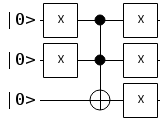
\includegraphics[scale=0.6]{resources/images/OR.png}
    \caption{Representation of OR gate using 1 Toffoli gate and 5 NOT gates}
    \label{fig:awesome_image}
\end{figure} 

For every AND and every OR in the classical circuit we are given, we will need one extra qubit. The extra qubit is always the third bit for the Toffoli gate. By using the quantum equivalents of the classical logic gates, and introducing extra qubits when necessary, we now have every part necessary to simulate the classical circuit on the quantum circuit such that the result of the classical circuit is produced by the quantum one. However, this is not yet our oracle.

At this point, we have a ciruit takes the input $\left | x \right \rangle \left | 0^{k} \right \rangle$ and gives $\left | junk(x) \right \rangle \left | f(x) \right \rangle$ where $f(x)$ is our classical search function. Note that where the previous state $x$ was, our circuit may modify the states of the qubits producing some new state that we call $junk(x)$. However, we need it to be of the form \cite{kothari12} 

$$\left | x \right \rangle \left | q \right \rangle \to \left | x \right \rangle \left | f(x) \oplus q \right \rangle$$

What this means is that we need to preserve the state of $\left | x \right \rangle$ through the circuit, reversing the result of $junk(x)$. To accomplish this, we can use a technique called ``uncomputation" for the quantum ciruit. Because every quantum gate is reversible, to get $\left | x \right \rangle$ back, we just have to perform all the gates we applied in backward order. However, before we do that, we ``copy" the result of the search function onto a new qubit using a CNOT gate. Then we can perform the uncomputation on the rest of the qubits, resulting in the desired form for the output.

At this point, the general steps for our algorithm are:

\begin{enumerate}
	\item Given an input function in the form of a classical circuit, we simulate each classical gate with a quantum gate, taking note of the order and which qubits we applied the gates to.
	\item Copy the output of the function, which should be the state of $n$th qubit, to an extra qubit.
	\item Perform the uncomputation by applying the same quantum gates we applied before but in the opposite order. 
\end{enumerate}

After we have achieved this circuit, we then need to complete the final step necessary for the oracle. By definition, the oracle flips the phase of the system state for a single input. This means that if the output qubit is in the $\left | 1 \right \rangle$ state, then we want to flip the phase of the state that produced. This can be done with one more extra qubit and a Pauli-z gate with a control on the ouput qubit.

However, we still have one final problem: the output qubit needs to be returned to its original state from before the oracle. The simplest way to return it to its original state is performing the simulated classical circuit once again. After this, we have will a quantum circuit that fully implements the oracle for Grover's algorithm.

\begin{figure}[H]
\begin{framed}
\textbf{To construct a circuit that implements the oracle for Grover's algorithm:}
\begin{enumerate}
\item Obtain a classical circuit, called $C_{c}$ that implements the desired search function using AND, OR and NOT gates.
\item Using quantum NOT and Toffoli gates, simulate the classical circuit with a quantum one, called $C_{q}$. (Note: for $N=2^n$ possible solutions to the search function, and $g$ classical gates, this quantum circuit will require $n+g$ qubits.)
\item Copy the output of this circuit to another qubit (called the output qubit) by using a quantum controlled NOT gate.
\item Using one more qubit, perform a Pauli-z gate on this extra qubit with a control on the output qubit. Note that the oracle function will require a total of $n+g+2=n_{q}$ qubits.
\item Apply $C_{q}$ again to return the output qubit back to its original state.
\end{enumerate}
\end{framed}
\end{figure}

My implementation in Scheme of this algorithm for generating the oracle can be seen in appendix C.

\section{Usage of Code}

The \textit{generate-fake-Oracle} function takes two arguments: the number of entries in the ``database" we are searching (must be a factor of 2), and the item we are searching for. It then outputs a the corresponding matrix which can be used as the oracle in Grover's algorithm.

\begin{lstlisting}
> (matrix-print (generate-fake-Oracle 4 2))
1 0 0 0 
0 1 0 0 
0 0 -1 0 
0 0 0 1 
\end{lstlisting}

The function \textit{Grover} simulates the algorithm. It takes one argument, the matrix representing the oracle function.

\begin{lstlisting}
> (Grover (generate-fake-Oracle 64 45))
The number of required qubits is 6
Number of operations required is 7
> (measure-register)
The most likely result is |101101> with a probability of 0.996585680786799
\end{lstlisting}

The function \textit{generate\-U\_omega} generates the oracle from a classical circuit. It a boolean expression as its only argument. After it is executed, the matrix representing the oracle operator will be set as \textit{U\_omega}, and \textit{input-qubits} will contain the number of input qubits (used later on). For example, for the boolean expression ($x_0 \land x_1$):

\begin{lstlisting}
> (generate-U_omega '(AND 0 1))
> (matrix-print U_omega)
1 0 0 0 0 0 0 0 0 0 0 0 0 0 0 0 0 0 0 0 0 0 0 0 0 0 0 0 0 0 0 0 
0 1 0 0 0 0 0 0 0 0 0 0 0 0 0 0 0 0 0 0 0 0 0 0 0 0 0 0 0 0 0 0 
0 0 -1 0 0 0 0 0 0 0 0 0 0 0 0 0 0 0 0 0 0 0 0 0 0 0 0 0 0 0 0 0 
0 0 0 1 0 0 0 0 0 0 0 0 0 0 0 0 0 0 0 0 0 0 0 0 0 0 0 0 0 0 0 0 
0 0 0 0 -1 0 0 0 0 0 0 0 0 0 0 0 0 0 0 0 0 0 0 0 0 0 0 0 0 0 0 0 
0 0 0 0 0 1 0 0 0 0 0 0 0 0 0 0 0 0 0 0 0 0 0 0 0 0 0 0 0 0 0 0 
0 0 0 0 0 0 1 0 0 0 0 0 0 0 0 0 0 0 0 0 0 0 0 0 0 0 0 0 0 0 0 0 
0 0 0 0 0 0 0 1 0 0 0 0 0 0 0 0 0 0 0 0 0 0 0 0 0 0 0 0 0 0 0 0 
0 0 0 0 0 0 0 0 1 0 0 0 0 0 0 0 0 0 0 0 0 0 0 0 0 0 0 0 0 0 0 0 
0 0 0 0 0 0 0 0 0 1 0 0 0 0 0 0 0 0 0 0 0 0 0 0 0 0 0 0 0 0 0 0 
0 0 0 0 0 0 0 0 0 0 -1 0 0 0 0 0 0 0 0 0 0 0 0 0 0 0 0 0 0 0 0 0 
0 0 0 0 0 0 0 0 0 0 0 1 0 0 0 0 0 0 0 0 0 0 0 0 0 0 0 0 0 0 0 0 
0 0 0 0 0 0 0 0 0 0 0 0 -1 0 0 0 0 0 0 0 0 0 0 0 0 0 0 0 0 0 0 0 
0 0 0 0 0 0 0 0 0 0 0 0 0 1 0 0 0 0 0 0 0 0 0 0 0 0 0 0 0 0 0 0 
0 0 0 0 0 0 0 0 0 0 0 0 0 0 1 0 0 0 0 0 0 0 0 0 0 0 0 0 0 0 0 0 
0 0 0 0 0 0 0 0 0 0 0 0 0 0 0 1 0 0 0 0 0 0 0 0 0 0 0 0 0 0 0 0 
0 0 0 0 0 0 0 0 0 0 0 0 0 0 0 0 1 0 0 0 0 0 0 0 0 0 0 0 0 0 0 0 
0 0 0 0 0 0 0 0 0 0 0 0 0 0 0 0 0 1 0 0 0 0 0 0 0 0 0 0 0 0 0 0 
0 0 0 0 0 0 0 0 0 0 0 0 0 0 0 0 0 0 -1 0 0 0 0 0 0 0 0 0 0 0 0 0 
0 0 0 0 0 0 0 0 0 0 0 0 0 0 0 0 0 0 0 1 0 0 0 0 0 0 0 0 0 0 0 0 
0 0 0 0 0 0 0 0 0 0 0 0 0 0 0 0 0 0 0 0 -1 0 0 0 0 0 0 0 0 0 0 0 
0 0 0 0 0 0 0 0 0 0 0 0 0 0 0 0 0 0 0 0 0 1 0 0 0 0 0 0 0 0 0 0 
0 0 0 0 0 0 0 0 0 0 0 0 0 0 0 0 0 0 0 0 0 0 1 0 0 0 0 0 0 0 0 0 
0 0 0 0 0 0 0 0 0 0 0 0 0 0 0 0 0 0 0 0 0 0 0 1 0 0 0 0 0 0 0 0 
0 0 0 0 0 0 0 0 0 0 0 0 0 0 0 0 0 0 0 0 0 0 0 0 -1 0 0 0 0 0 0 0 
0 0 0 0 0 0 0 0 0 0 0 0 0 0 0 0 0 0 0 0 0 0 0 0 0 1 0 0 0 0 0 0 
0 0 0 0 0 0 0 0 0 0 0 0 0 0 0 0 0 0 0 0 0 0 0 0 0 0 1 0 0 0 0 0 
0 0 0 0 0 0 0 0 0 0 0 0 0 0 0 0 0 0 0 0 0 0 0 0 0 0 0 1 0 0 0 0 
0 0 0 0 0 0 0 0 0 0 0 0 0 0 0 0 0 0 0 0 0 0 0 0 0 0 0 0 1 0 0 0 
0 0 0 0 0 0 0 0 0 0 0 0 0 0 0 0 0 0 0 0 0 0 0 0 0 0 0 0 0 1 0 0 
0 0 0 0 0 0 0 0 0 0 0 0 0 0 0 0 0 0 0 0 0 0 0 0 0 0 0 0 0 0 -1 0 
0 0 0 0 0 0 0 0 0 0 0 0 0 0 0 0 0 0 0 0 0 0 0 0 0 0 0 0 0 0 0 1 
> input-qubits
1
\end{lstlisting}

Besides the \textit{AND} operator, there is also the \textit{OR} and the \textit{NOT} operators. Both \textit{AND} and \textit{OR} take exactly two arguments, while \textit{NOT} takes one.

Because there are extra qubits required for the simulated circuit (notice that in the above example, 5 qubits are needed despite there only being two inputs), there is a special Grover's algorithm function called `Grover-from-classical-circuit` that takes this into account. To use it, input the \textit{U\_omega} and \textit{input-qubits} which are automatically generated after using \textit{generate-U\_omega}.

\begin{lstlisting}
> (Grover-from-classical-circuit U_omega input-qubits)
The number of required qubits is 5
Number of operations required is 2
> (measure-register)
The most likely result is |11000> with a probability of 0.9999999999999987
\end{lstlisting}

Since the solution to the classical circuit we inputted is $\Ket{11}$ we can see that the algorithm was successful. Note that Grover's algorithm expects that there is only one state of the input bits which flips the phase. This means there should only be one solution to the search function, and thus just one solution to the classical circuit inputted. If there is more than one, \textit{generate-U\_omega} will not output a valid oracle matrix.

\section{Conclusion}

By representing a quantum computer as a series of matrix operations, I was able to successfully simulate quantum computation as well as perform Grover's algorithm. Furthermore, I was able to come up with a simple algorithm for generating a quantum circuit of only common quantum gates that simulates a given classical circuit. As this is a necessary step in order to use Grover's algorithm in a real world situation, this demonstrates how quantum computers might be used in the future. In the next chapter, I show how to implement an adaption of Grover's algorithm to the problem of associative memory.


\chapter{Implementing Associative Memory on a Quantum Computer Simulator}

\section{Introduction}

Associative memory deals with the problem of ``learning" a set of patterns, and then being able to ``recall" a certain pattern when presented with just a part of the pattern. There are many simple classical algorithms that can achieve this task, such as storing the patterns in a database and then searching over the database (and each pattern) to find the one that matches. However, these can be slow and require lots of storage space. Another classical solution to this problem is using a Hopfield network, a type of neural network which can be used to implement associative memory. However, if the patterns are of length $n$, the neural network requires $n$ neurons, and is then limited in how many patterns it can store (usually less than half of $n$).

Quantum computing allows a significant improvement over neural network techniques. Dan Ventura and Tony Martinez, in a paper titled \textit{Quantum Associative Memory}, present two algorithms that achieve associative memory that allow up to $m=2^n$ patterns to be stored on $n$ qubits in a \textit{training} phase, which can then later be \textit{recalled} in another phase of the overall algorithm. Here, training refers to the stage of the algorithm where the patterns are ``learned" and stored on the quantum computer in some capacity, and recall refers to the part where a portion of a pattern is presented and the quantum computer responds with a matching pattern that was previously stored. The overall algorithm has a training complexity of $O(mn)$ and a recall complexity of $O(\sqrt{n})$ \cite{Ven00}. 

In order to show how this algorithm might actually be implemented on a universal quantum computer, each stage of Ventura's and Martinez's (V\&M) paper was achieved and simulated using only common quantum gates. Unless noted, all parts of the algorithms are taken directly from their paper.

\section{Explanation of Algorithms}

\subsection{Overview}

Given a set $P$ of patterns to be learned, each pattern is loaded one at a time onto the $n$ qubits until the system state has an equal distribution of all the patterns present. A slightly modified Grover's algorithm can then be used to retrieve a pattern based on a known portion of it.

\subsection{Learning Stage}

For patterns of length $n$, $n$ qubits are needed to store the pattern (called the storage qubits). However, during the learning stage, three extra qubits are necessary: one as an intermediate qubit which is always returned to $ \left | 0 \right \rangle$ (called $g$), and two as control qubits (called $c_1$ and $c_2$). Note that this is a slight modification of V\&M's algorithm, which required $2n+2$ qubits. This is because I used a Z-gate with controls on every one of the storage bits for the sake of much shorter simulation times.\footnote{Any single qubit gate U with an arbitrary number of controls can be achieved by using a series of CNOT gates and twice the qubits.} For the algorithm, we require two special gates:

$$\mathrm{C0NOT}=\begin{pmatrix}
0 & 1 & 0 & 0 \\
1 & 0 & 0 & 0 \\
0 & 0 & 1 & 0 \\
0 & 0 & 0 & 1 \\
\end{pmatrix}$$

$$\mathrm{CS_p}=\begin{pmatrix}
1 & 0 & 0 & 0 \\
0 & 1 & 0 & 0 \\
0 & 0 & \sqrt{\frac{p-1}{p}} & \frac{-1}{\sqrt{p}} \\
0 & 0 & \frac{1}{\sqrt{p}} & \sqrt{\frac{p-1}{p}} \\
\end{pmatrix}$$

C0NOT is simply a controlled-not gate that flips the second bit if the first is in the $\ket{0}$ state, instead of $\ket{1}$. It can be constructed by doing a NOT on the first qubit, a CNOT, and then another NOT on the first.

$\mathrm{CS_p}$ allows us to slice the state with the control bit as a one into two states, one being $\frac{1}{n}$ of the superposition, and the other being $\frac{p}{n}$ of the superposition.\footnote{A better and more in depth explanation of how this gate works can be found in V\&M's paper.}

Here are the steps of the algorithm for each pattern in $P$:

\begin{framed}
\textbf{Learning a single pattern on $n$ qubits:}
\begin{enumerate}
	\item Apply C0NOT gates with a control on $c_2$ to storage qubit if the corresponding bit in the pattern is a 1.
	\item Apply CNOT gate with control on $c_2$ to $c_1$.
	\item Apply $\mathrm{CS_p}$ with control on $c_1$ onto $c_2$, where $p$ is the number of patterns remaining including the pattern being learned.
	\item Apply NOT gates to every qubit where the corresponding bit in the pattern is a 0.
	\item Apply CNOT gate with controls on every storage qubit to $g$.
	\item Apply CNOT gate with control on $g$ to $c_1$.
	\item Repeat step 5.
	\item Repeat step 4.
\end{enumerate}
\end{framed}

We can repeat this algorithm for every pattern until $P$ has been ``learned" by the quantum computer. By the end of the algorithm, all three extra qubits, $g$, $c_1$ and $c_2$, will be unentangled from the rest of the system so we can safely discard them.

Note that is single pattern learning algorithm is $O(n)$, and as we must apply it for $m$ patterns, the entire learning algorithm is $O(mn)$.

\begin{figure}[!htb]
\centering
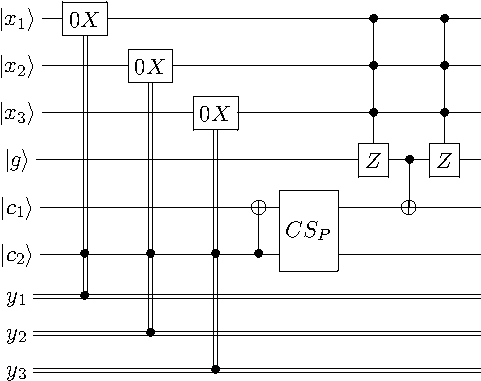
\includegraphics[width=0.5\textwidth]{resources/pdfs/assoc1-crop.pdf}
\caption{This example is for loading patterns with a length of 3. The pattern would come in loaded on the classical bits, $y_1$, $y_2$ and $y_3$. The 0X gate represents a controlled NOT except that the control looks for a zero on $c2$.}
\label{fig:digraph}
\end{figure}

\subsection{Recall algorithm}

As previously stated, the recall algorithm uses a modified Grover search to find the correct learned pattern. The first difference is that we do not prepare the system in any way by applying Hadamard gates at the beginning, as we already have the superposition we want. The second is that at the beginning, since the Grover diffusion operator will also flip the phases of all the states representing the patterns (instead of just the desired pattern), we need another operator that flips all the phases of the patterns back. We call this operator $I_P$. In terms of its matrix, it can be represented as an identity matrix where the $i$th 1 is changed to a $-1$ if $i$ is the decimal representation of one of the patterns. We can construct it with gates by going through every pattern, applying a NOT gate on the qubits that correspond to zeros in the pattern, applying a controlled Pauli-z gate with controls on every qubit (except the one with the Pauli-z gate, which can be any of them), and then re-applying the same NOT gates. This method can be seen in the function \textit{constr-patterns-phaser} in my code. We will notate the normal Grover diffusion operator with $G$.

\begin{figure}[!htb]
\centering
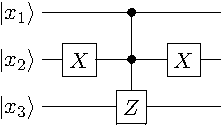
\includegraphics[width=0.25\textwidth]{resources/pdfs/assoc2-crop.pdf}
\caption{This example represents one pattern for $I_P$. The pattern would be (1 0 1), so we need to apply the NOT gate to the second qubit because it is a zero.}
\label{fig:digraph2}
\end{figure}

We want the oracle for Grover's algorithm to be a quantum circuit which flips the phase of the system if it is in the correct pattern. Thus, we can construct it simply by applying NOT gates to all qubits that correspond to zeros in the part of the pattern we know, applying a controlled Pauli-z gate with controls on all the qubits corresponding to bits we know onto one of the qubits corresponding to the qubits we do not know, and then applying the same NOT gates again. This method can be seen in the function \textit{constr-search-phaser} in my code. We will notate this oracle function with $I_s$.


\begin{figure}[!htb]
\centering
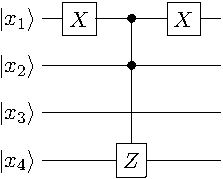
\includegraphics[width=0.25\textwidth]{resources/pdfs/assoc3-crop.pdf}
\caption{This example would correspond to the partial sequence (0 1 ? ?). We apply a NOT gate to the first qubit because we know it is a zero, then a Z with controls on the known qubits with a target on one of the unknowns, and then re-apply the NOT.}
\label{fig:digraph3}
\end{figure}

\begin{framed}
\textbf{Recalling pattern given partial sequence }
\begin{enumerate}
	\item Apply $I_sGI_PG$ to the qubits.
	\item Repeat $T$ times:
	\begin{enumerate}
		\item Apply $I_sG$ to the qubits.
	\end{enumerate}
	\item Measure register.
\end{enumerate}
\end{framed}

Where $$T=\frac{\frac{\pi}{2}-\arctan \left (\frac{k}{l}\sqrt{\frac{r_0+r_1}{N-r_0-r_1}} \right )}{\arccos \left ( 1-2\frac{r_0+r_1}{N} \right )}$$

and

$$k=4a-ab+\frac{r_1}{r_0+r_1}$$
$$l=-ab+\frac{2a(N+p-r_0-2r_1)}{N-r_0-r_1}-\frac{p-r_1}{N-r_0-r_1}$$
$$a=\frac{2(p-2r_1)}{N}$$
$$b=\frac{4(p+r_0)}{N}$$

where $p$ is the number of patterns, $r_0$ is the number of marked states (states involving the unknown qubits that the controlled Pauli-z gates in $I_P$ did not act on, or, in the matrix representation, all the states corresponding to the $-1$s in the matrix) that do not correspond to learned patterns, and $r_1$ all the marked states that do correspond to learned states. In my code, I assumed that there was only one learned state that the recall should return, so I assumed $r_1$ is 1 and $r_0$ is equal to $2^u-1$ where $u$ is the number of unknowns in the partial sequence.

Though I have no understanding of $T$, V\&M assert that the second algorithm is still $O(\sqrt{n})$ and the same as Grover's algorithm. This makes sense in that though it was modified slightly, the algorithm remains essentially the same.

\section{Implementation and Usage}
The implementation of quantum associative memory written for my quantum computer simulator has been included in appendix D. The learning algorithm is called \textit{learn}, and the recall algorithm is called \textit{Grover-part}. They can be used like so:
	
	\begin{lstlisting}
	> (define P '((0 0 0 0) (0 0 1 1) (0 1 1 0) (1 0 0 1) (1 1 0 0) (1 1 1 1)))
	> (learn P)
	> (Grover-part '(0 1 1 ?) P)
	> (measure-register)
	The most likely result is |0110> with a probability of 0.8437500000000002
	\end{lstlisting}

\section{Discussion and Conclusion}

Though in general I was able to successfully implement most parts of the algorithms outlined by V\&M, there was one notable issue that I had: The calculation of $T$ often gave me the wrong value. As a result, the code would often apply the oracle and Grover diffusion operator too many times and thus the final superposition was not likely to return the correct value. For example, when 6 patterns of length 4 are learned, and a partial sequence with two unknowns is used to recall, V\&M's definition of $T$ gives $T=3$. However, repeating the Grover step results in a final superposition with a $\approx 26\%$ chance of returning one of the incorrect patterns, and only a $\approx 9\%$ chance of retrieving the correct pattern. If we set $T=0$, however, the final system state has a $\approx84\%$ chance of returning the correct pattern. While this may be due to a mistake in my implementation of it, I have always been able to achieve a high rate of getting back the correct pattern using different values of $T$, which suggests there is an issue with my (or V\&M's) calculation of $T$.

In the next chapter, I discuss the quantum Fourier transform and how to achieve it with simple quantum gates.

\chapter{The Quantum Fourier Transform}

\section{Overview}
The discrete Fourier transform (DFT) is a function which takes a ``signal" in time space and breaks it down into its constituent frequencies, such that if we were to add up all of those produced frequencies, we would return to the original signal. For example, we could record some music by recording regular samples of the sound signal, and then use the DFT to examine which sound frequencies were present and their amplitudes. The DFT has wide ranging applications from music to radio astronomy.

\section{QFT with a Matrix}

The quantum Fourier transform is the unitary discrete Fourier transform on the state of the quantum computer. The classical unitary discrete Fourier transform is defined as a map $F: \mathbb{C}^N \to \mathbb{C}^N$ where $N = 2^n$ and
$$x_k \to \frac{1}{\sqrt{N}}\sum_{m = 0}^{N - 1}e^{2\pi i k \frac{m}{N}} x_m$$
where $x$ is a vector of the samples. Note that this is slightly different than the classical DFT as defined in the previous section because it is unitary, and so it preserves the inner product of two valid vectors as input. In this case, it just means normalizing the output with a factor of $\frac{1}{\sqrt{2}}$. 

The quantum version is almost exactly the same, except that we transform quantum states to other quantum states according to the function
$$\Ket{x_k} \to \frac{1}{\sqrt{N}}\sum_{m = 0}^{N - 1}e^{2\pi i k \frac{m}{N}} \Ket{x_m}$$
where $\Ket{x_k}$ is the current complex magnitude of state $\Ket{k}$. Now let $\omega = e^{2\pi i /N}$ (leaving it as just $\omega$ when the $N$ value is obvious), we can simplify this to
$$\Ket{x_k} \to \frac{1}{\sqrt{N}}\sum_{m = 0}^{N - 1}\omega^{km} \Ket{x_m}$$

$$\begin{pmatrix}
	x_0 \\
	x_1 \\
	x_2 \\
	\vdots \\
    x_k \\
    \vdots \\
    x_{N-1}
  \end{pmatrix}
\to \frac{1}{\sqrt{N}}
  \begin{pmatrix}
	\sum_{m=0}^{N-1} \omega^{0\cdot m} x_m\\
	\sum_{m=0}^{N-1} \omega^{m} x_m \\
	\sum_{m=0}^{N-1} \omega^{2m} x_m \\
	\vdots \\
    \sum_{m=0}^{N-1} \omega^{km} x_m \\
    \vdots \\
    \sum_{m=0}^{N-1} \omega^{(N-1)m} x_m
  \end{pmatrix}
$$

As we can see, each value in the resulting vector is a linear combination of the values of the original quantum state. This suggests that it is both a valid quantum transformation (as all quantum transformations should be linear and reversible) and that we can represent it as a matrix multiplication. In fact, it is easy to see how the matrix will work: each row should pertain to a different sequence of rotations. The first row should be simply be all 1s, as the first value of the resulting vector is just a sum of all the original states. In other words, it should not rotate the original values at all, meaning it should look like $\omega^0, \omega^0, ... ,\omega^0 = 1, 1, ..., 1$. The next row should be the sequence of increasing powers of $\omega$, as $k = 1$. This should look like $\omega^0, \omega^1, \omega^2, ... \omega^{N-1}$. The next row should be a sequence of $\omega$ where the power goes up by two every time (because $k = 2$), so $\omega^0, \omega^2, \omega^4, ... \omega^{2(N-1)}$. Following this pattern gives us the matrix which performs the DFT on a quantum state:

$$F_N = \begin{pmatrix}
  \omega^0 & \omega^0 & \omega^0 & \omega^0 & \cdots & \omega^0 \\
  \omega^0 & \omega^1 & \omega^2 & \omega^3 & \cdots & \omega^{N-1} \\
  \omega^0 & \omega^2 & \omega^4 & \omega^6 & \cdots & \omega^{2(N-1)} \\
  \omega^0 & \omega^3 & \omega^6 & \omega^9 & \cdots & \omega^{3(N-1)} \\
  \vdots & \vdots & \vdots & \vdots & \ddots & \vdots \\
  \omega^0 & \omega^{N-1} & \omega^{2(N-1)} & \omega^{3(N-1)} & \cdots & \omega^{(N-1)(N-1)}
  \end{pmatrix}$$

\section{Gate-Based QFT}
We have shown that we can construct a valid matrix operator that performs the QFT on any quantum state. However, this does not tell us very much about how one would go about actually constructing the machine that would perform this. To show this, as well as to demonstrate how well the algorithm will run on a quantum computer, we want to break down the transformation into a series of simple quantum gates.

Luckily, the QFT can be easily broken down into simple quantum gates. In fact, we can define the set up of the gates recursively: as long as we have the series of gates the works on $n-1$ qubits, it is easy to produce the next gates which compute it on $n$ qubits.


\subsection{Single Qubit Case}
We will start with the case of performing the QFT on a single qubit. We want to find a series of gates which performs
$$\ket{q_0} \to F_2\ket{q_0} = \frac{1}{\sqrt{2}}\begin{pmatrix}\omega^0 & \omega^0 \\ \omega^0 & \omega^1 \end{pmatrix} \Ket{q_0} = \frac{1}{\sqrt{2}}\begin{pmatrix}1 & 1 \\ 1 & -1 \end{pmatrix} \Ket{q_0}.$$
Immediately, we recognize that $F_2$ has the exact same matrix representation as the Hadamard gate. In fact, the Hadamard transform is exactly $F_2$, the QFT on a single qubit.
  
\begin{figure}[h]
\centering
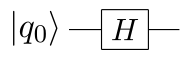
\includegraphics[width=0.2\textwidth]{resources/images/hadamard.png}
\caption{\label{fig:Hadamard}The QFT on a single qubit consists of a single Hadamard gate.}
\end{figure}

\subsection{Recursive Case}
Now let us consider the case where we already have a circuit which performs the QFT on $n-1$ qubits and we want to use this to build one which performs the QFT on $n$ qubits. To do this, we will first simplify the problem by assuming that our original quantum state is actually a classical state, meaning that every qubit is equal to either $\Ket{0}$ or $\Ket{1}$. In this case, if the original state is equal to $\Ket{j}$, the QFT is reduced to

$$\begin{pmatrix}
	x_0 \\
	x_1 \\
	x_2 \\
	\vdots \\
    x_k \\
    \vdots \\
    x_{N-1}
  \end{pmatrix}
\to \frac{1}{\sqrt{N}}
  \begin{pmatrix}
	\sum_{m=0}^{N-1} \omega^{0\cdot n} x_m\\
	\sum_{m=0}^{N-1} \omega^{m} x_m \\
	\sum_{m=0}^{N-1} \omega^{2m} x_m \\
	\vdots \\
    \sum_{m=0}^{N-1} \omega^{km} x_m \\
    \vdots \\
    \sum_{m=0}^{N-1} \omega^{(N-1)m} x_m
  \end{pmatrix} = 
  \frac{1}{\sqrt{N}}
  \begin{pmatrix}
	1\\
	\omega^{j} \\
	\omega^{2j} \\
	\vdots \\
    \omega^{kj} \\
    \vdots \\
    \omega^{(N-1)j}
  \end{pmatrix}
$$

Note that this is because every value of $x$ vector is 0 except at the single index $j$ where $x_j = 1$, meaning that all the sums in the transform will simplify to just $\omega^{kj}$.
We can then break this final state down into the tensor products of the individual qubit states after the transform. First notice that 
$$\frac{1}{\sqrt{N}}
  \begin{pmatrix}
	1\\
	\omega^{j} \\
	\omega^{2j} \\
	\vdots \\
    \omega^{kj} \\
    \vdots \\
    \omega^{(N-1)j}
  \end{pmatrix} = 
  \frac{1}{\sqrt{N}}
  \qcol{1}{\omega^{2^{n-1}j}}
  \otimes
  \qcol{1}{\omega^{2^{n-2}j}}
  \otimes \cdots \otimes
  \qcol{1}{\omega^{2j}}
  \otimes
  \qcol{1}{\omega^{j}}
$$

We now assume that we already have a circuit which performs this transform on $n-1$ qubits, except that the output is completely reversed. Let $\hat{\omega} = \omega_{n-1}$. Now the output of just this circuit becomes 

$$\frac{1}{\sqrt{2^{n-1}}} 
  \qcol{1}{\hat{\omega}^{j_*}}
  \otimes
  \qcol{1}{\hat{\omega}^{2j_*}}
  \otimes \cdots \otimes
  \qcol{1}{\hat{\omega}^{2^{n-3}j_*}}
  \otimes
  \qcol{1}{\hat{\omega}^{2^{n-2}j_*}}$$
  
instead, where $j_*$ is the $j$ state but with the bits in reverse order as well. Because $\hat{\omega}^{k} = e^{2\pi i k / 2^{n-1}} = e^{(2k) 2\pi i / 2^n} = \omega^{2k}$, we can rewrite this as
$$\frac{1}{\sqrt{2^{n-1}}} 
  \qcol{1}{\omega^{2j_*}}
  \otimes
  \qcol{1}{\omega^{2\cdot2j_*}}
  \otimes \cdots \otimes
  \qcol{1}{\omega^{2\cdot2^{n-3}j_*}}
  \otimes
  \qcol{1}{\omega^{2\cdot2^{n-2}j_*}}.$$
  
We now introduce another qubit $q_0$ in a classical state, and apply our assumed QFT on the $n-1$ following qubits. This leaves us with the following state:
$$\frac{1}{\sqrt{2^{n-1}}} 
  \qcol{1}{\omega^{2j_*}}
  \otimes
  \qcol{1}{\omega^{2\cdot2j_*}}
  \otimes \cdots \otimes
  \qcol{1}{\omega^{2\cdot2^{n-3}j_*}}
  \otimes
  \qcol{1}{\omega^{2\cdot2^{n-2}j_*}}
  \otimes q_{n-1}.$$
  
\begin{figure}[h]
\centering
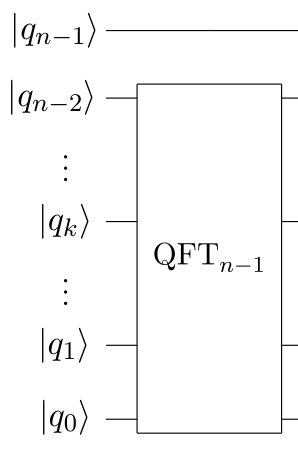
\includegraphics[width=0.25\textwidth]{resources/images/qft1.png}
\caption{\label{fig:qft1}The reverse order QFT on qubits 1 through $n-1$.}
\end{figure}

Let the state of $q_n$ be $\Ket{b}$ where $b$ is either 0 or 1. If the state of the first $n-1$ qubits is $\Ket{j}$, then the new state is $\Ket{j + 2^nb}$, because we inserted $q_{n-1}$ at the end of the sequence.

We now make the crucial step: we use a series of controlled phase gates to rotate the first $n-1$ qubits by the correct amount if $b = 1$. A controlled phase gate $CR_\theta$ on two qubits, with a control on the first, rotates the second qubit by $\theta$ radians. It is represented by the matrix

$$CR_\theta = \begin{pmatrix}
1 & 0 & 0 & 0 \\
0 & 1 & 0 & 0 \\
0 & 0 & 1 & 0 \\
0 & 0 & 0 & e^{i\theta}
\end{pmatrix}$$

If we use a series of these gates, always placing the control on the $n$th qubit and then rotating the first qubit by $2\pi/N$ radians, the second qubit by $2\cdot 2\pi/N$ radians, the third by $3\cdot 2\pi/N$ radians and so on, we will be left with following quantum state:

$$\frac{1}{\sqrt{2^{n-1}}} 
  \qcol{1}{\omega^{2j_*}\omega^{b}}
  \otimes
  \qcol{1}{\omega^{2\cdot2j_*}\omega^{2b}}
  \otimes \cdots \otimes
  \qcol{1}{\omega^{2\cdot2^{n-3}j_*}\omega^{(n-1)b}}
  \otimes
  \qcol{1}{\omega^{2\cdot2^{n-2}j_*}\omega^{nb}}
  \otimes q_{n-1}$$
$$= \frac{1}{\sqrt{2^{n-1}}} 
  \qcol{1}{\omega^{2j_* + b}}
  \otimes
  \qcol{1}{\omega^{2(2j_* + b)}}
  \otimes \cdots \otimes
  \qcol{1}{\omega^{2^{n-3}(2j_* + b)}}
  \otimes
  \qcol{1}{\omega^{2^{n-2}(2j_* + b)}}
  \otimes q_{n-1}$$
  
Because the bit reversal of $2j_* + b$ is $j + 2^nb$, if we let $p = j + 2^nb$, we can write the state as
$$= \frac{1}{\sqrt{2^{n-1}}} 
  \qcol{1}{\omega^{p_*}}
  \otimes
  \qcol{1}{\omega^{2p_*}}
  \otimes \cdots \otimes
  \qcol{1}{\omega^{2^{n-3}p_*}}
  \otimes
  \qcol{1}{\omega^{2^{n-2}p_*}}
  \otimes q_{n-1}$$

\begin{figure}[h]
\centering
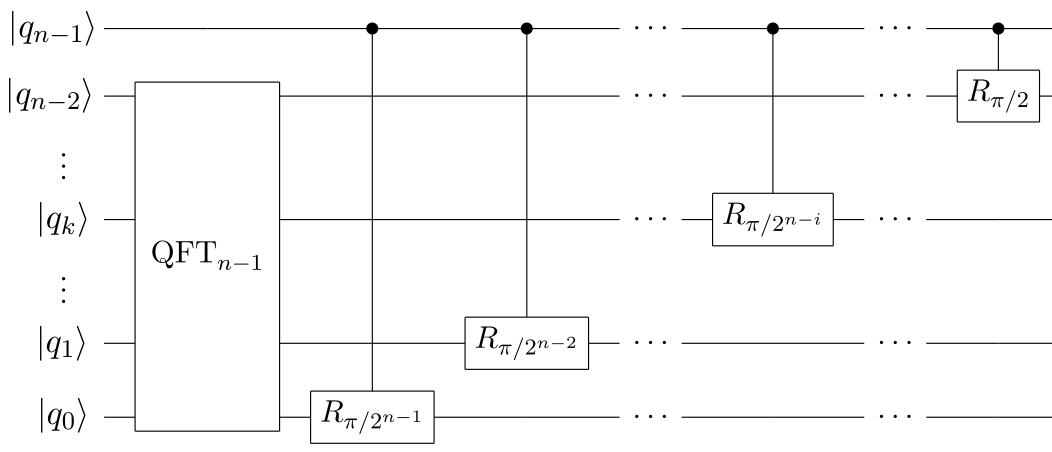
\includegraphics[width=0.9\textwidth]{resources/images/qft2.png}
\caption{\label{fig:qft2}The next stage of the circuit. The solid dots represent where the control of the phase gates is placed.}
\end{figure}


The final step we need to take is then put the final qubit, $q_{n-1}$, into the correct state. We know it should be in the state
$$\qcol{1}{\omega^{2^{n-1}p_*}} = \qcol{1}{e^{2\pi i 2^{n-1}p_* / 2^n}} = \qcol{1}{e^{\pi i p_*}} = \qcol{1}{e^{\pi i (b + 2j_*)}} = \qcol{1}{e^{\pi i b}}$$

We can easily accomplish this in the exact same way as in the single qubit case: a single Hadamard gate. We know that
$$H\Ket{0} = \frac{1}{\sqrt{2}}\begin{pmatrix}
1 & 1\\
1 & -1
\end{pmatrix} \qcol{1}{0} = \frac{1}{\sqrt{2}} \qcol{1}{1}$$
and that
$$H\Ket{1} = \frac{1}{\sqrt{2}}\begin{pmatrix}
1 & 1\\
1 & -1
\end{pmatrix} \qcol{0}{1} = \frac{1}{\sqrt{2}} \qcol{1}{-1}$$

This means if we apply the Hadamard gate to qubit $q_0$, whose state is $\Ket{b}$, we get
$$H\Ket{b} = \frac{1}{\sqrt{2}} \qcol{1}{-1^b} = \frac{1}{\sqrt{2}} \qcol{1}{e^{\pi i b}}$$

\begin{figure}[h]
\centering
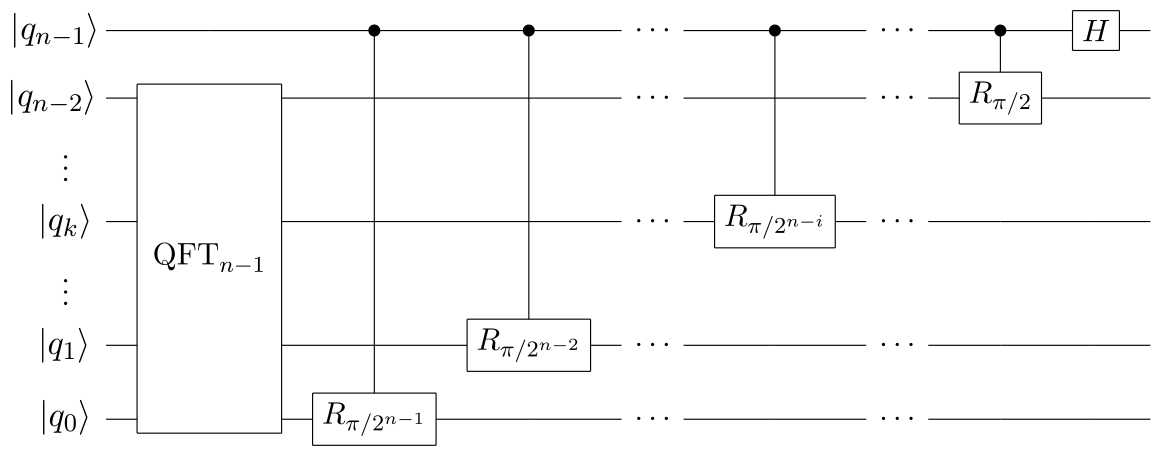
\includegraphics[width=1\textwidth]{resources/images/qft3.png}
\caption{\label{fig:qft3}The final stage of the circuit, with a Hadamard on the final qubit.}
\end{figure}

Putting this altogether, we get a circuit which will result in the state
$$\frac{1}{\sqrt{2^{n-1}}} 
  \qcol{1}{\omega^{p_*}}
  \otimes
  \qcol{1}{\omega^{2p_*}}
  \otimes \cdots \otimes
  \qcol{1}{\omega^{2^{n-3}p_*}}
  \otimes
  \qcol{1}{\omega^{2^{n-2}p_*}}
  \otimes
  \frac{1}{\sqrt{2}} \qcol{1}{e^{\pi i b}}$$
  
$$= \frac{1}{\sqrt{N}}
  \qcol{1}{\omega^{p_*}}
  \otimes
  \qcol{1}{\omega^{2p_*}}
  \otimes \cdots \otimes
  \qcol{1}{\omega^{2^{n-3}p_*}}
  \otimes
  \qcol{1}{\omega^{2^{n-2}p_*}}
  \otimes
  \qcol{1}{\omega^{2^{n-1}p_*}}$$

This is thus the result of the QFT with the order of the qubits reversed. Because we have shown that we can do the QFT on a single qubit using a Hadamard gate (noting the reverse ordering is the same in the single qubit case), and that if we have a circuit which implements the reverse qubit order QFT on $n-1$ qubits we can get the reverse order QFT on $n$ qubits, we have shown that we can make a circuit implementing the reverse order QFT on any $n$ qubits as long as the qubits are in an initially classical state.

We also know that we can swap the state of any two qubits using a \textit{SWAP} gate, defined as
$$\textit{SWAP} = \begin{pmatrix}
1 & 0 & 0 & 0\\
0 & 0 & 1 & 0\\
0 & 1 & 0 & 0\\
0 & 0 & 0 & 1
\end{pmatrix}.$$

Thus, if it is needed to have a circuit for which the result is in the correct order, we can simply use \textit{SWAP} gates to obtain the result of the true QFT. This can be done by first reversing the order of the qubits using \textit{SWAP} gates, and then running the reverse order QFT circuit as defined above.

Finally, we conclude that though we started with the assumption that the qubits were in a classical state, the circuit we came up with will work for any starting quantum state. This is first because any quantum state is a linear combination of all the possible classical states, that is any quantum state $\Ket{\Psi}$ with $n$ qubits can be written as
$$\Ket{\Psi} = \alpha_0\Ket{0} + \alpha_1\Ket{1} + \alpha_2\Ket{2} + ... + \alpha_{n-1}\Ket{n-1}$$
where all $\alpha_k \in \mathbb{C}$. Secondly, because we made sure to only use valid quantum gates in the construction of our QFT circuit, we know that the circuit is also simply a linear transformation of the original state. This means we can think of our circuit simply doing the QFT on each of classical states present in the original state in proportion to each state's magnitude (where $\alpha_k$ is the magnitude of state $\Ket{k}$).

To motivate this, we can simply use matrix multiplication on each of the matrix forms of the different gates we used in our circuit to see what the overall function is on two qubits (noticing that we must do this in reverse order of how we apply the gates):

$$(H \otimes I_2)CR_{\pi/2}(I_2 \otimes H)\textit{SWAP}$$
$$= \frac{1}{\sqrt{2}}\begin{pmatrix}
1 & 0 & 1 & 0 \\
0 & 1 & 0 & 1 \\
1 & 0 &-1 & 0 \\
0 & 1 & 0 &-1
\end{pmatrix}
\begin{pmatrix}
1 & 0 & 0 & 0 \\
0 & 1 & 0 & 0 \\
0 & 0 & 1 & 0 \\
0 & 0 & 0 & i
\end{pmatrix}
\frac{1}{\sqrt{2}}\begin{pmatrix}
1 & 1 & 0 & 0 \\
1 &-1 & 0 & 0 \\
0 & 0 & 1 & 1 \\
0 & 0 & 1 &-1
\end{pmatrix}
\begin{pmatrix}
1 & 0 & 0 & 0\\
0 & 0 & 1 & 0\\
0 & 1 & 0 & 0\\
0 & 0 & 0 & 1
\end{pmatrix}$$
$$=\frac{1}{2} \begin{pmatrix}
1 & 1 & 1 & 1 \\
1 & i & -1 & -i \\
1 & -1 & 1 & -1 \\
1 & -i & -1 & i
\end{pmatrix} = F_4.$$

Thus we can confirm our circuit works in this case. Here is an example of the full circuit for 4 qubits:

\begin{center}
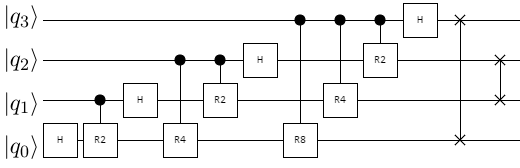
\includegraphics[width=0.7\textwidth]{resources/images/qft4.png}
\end{center}

Note that here the X gates are swap gates and R2, R4 and R8 gates correspond to $CR_{\pi/2}$, $CR_{\pi/4}$ and $CR_{\pi/8}$ respectively.

\section{Conclusion}
The QFT is surprisingly efficient. In the $k$th recursive stage of the QFT, we use exactly $k$ gates ($k-1$ controlled phase gates and one Hadamard). This means that overall, we use $1 + 2 + 3 + ... + n = \frac{n(n+1)}{2} = O(n^2)$ operations (generally, the \textit{SWAP} gates are not counted as they are not necessary). However, there exist even more efficient implementations of the QFT using only $O(n\log n)$ gates.

One important difference between the QFT and the classical DFT is that the QFT runs on quantum states and produces the result of the transform as quantum state, meaning that we would not be able to examine exactly what the result of the transform was. This we run into the fundamental problem that we can only ``measure" a quantum state, meaning that it collapses to a single classical value and the rest of the quantum information is lost. However, the QFT still plays a very important role as a subroutine of other quantum algorithms. One notable one is that the QFT is a part of Shor's algorithm which is the best known factoring algorithm.

In the next chapter, I explain a different model of quantum computing called quantum annealing, and explain how it can be used to solve a certain type of physics problem.

\chapter{Embedding 3D Lattice Ising Problems on the D-Wave Processor}
\section{Introduction to the Ising Model}
The Ising Model is a mathematical model inspired by ferromagnets in physics. Ising problems consist of a selection of $n$ discrete spin variables ($s = [s_0, s_1, ..., s_{n-1}]$, a vector of length $n$), weights placed on each variable ($h = [h_0, h_1, ..., h_{n-1}]$, a vector of length $n$), and weights on each pair of variables ($J$, an $n*n$ matrix). Note that the diagonal entries of $J$ have no effect, and that $J_{ij}=J_{ji}$. For every spin variable $s_k \in s$, $s_k \in \{-1,1\}$. The energy for a problem $h$ and $J$ and a given spin state $s$ is given by

$$E(s) = \sum h_is_i + \sum_{i,j>i}J_{ij}s_is_j.$$

Our aim is to find good ways of finding low energy states for a given problem $h$ and $J$. If we are able to find a state that has the lowest possible energy, or the \textit{ground energy}, it is called a \textit{ground state}.

Generally, the \textit{dimension} of an lattice Ising problem is understood to be the dimension of the lattice, not of the connectivity graph itself. This means a 1-dimensional lattice problem is a string with a connection between consecutive qubits, a 2-dimensional problem is a grid where each variable is connected to its four neighbors, and so on. It is worth noting that lattice Ising problems of greater that 2 dimensions have shown to be NP-hard, making the problem interesting for both physicists looking for good ways of making models as well as computer scientists.

\section{Simulated annealing}
Simulated annealing is a simple but effective heuristic algorithm for solving Ising problems. It is inspired by the physical annealing process. Physicists noted that if one takes a hot ferromagnet, applies a magnetic field, and then cools it very quickly, the magnetic particles end up in a state of disorder similar to what would be found in its hot state. However, if it is cooled slowly, then the particles will align themselves during the cooling process resulting in a well-ordered magnet by the end. This process is called annealing.

Simulated annealing takes this idea and attempts to replicate it. It is a Metropolis algorithm, meaning small changes are made to the system state and accepted if they improve the energy. However, even if the change results in a higher energy state, simulated annealing will accept the change with a certain probability which is a function of temperature. Over the course of the algorithm, we slowly lower the temperature, meaning worse states will have a higher likelihood of being accepted towards the beginning of the anneal than at the end. This concept allows simulated annealing to work itself out of local minima at the beginning, and then slowly settle in to the minimum it finds itself in at the end.

Given a state $s$ with $n$ spins, a new state $s'$, and the current temperature $T$, simulated annealing will accept the new state with probability
$$P(s, s', T) = e^{-(E(s')-E(s))/T}$$

Usually, this Metropolis update will be applied a fixed number of times. The entire anneal is divided up into \textit{sweeps}, where in each sweep the Metropolis update is applied to every variable in a random ordering.

An overview of simulated as applied to the Ising model is as follows:

\begin{figure}[H]
Input: $\beta_i, \beta_f, M, h, J$. (the $\beta$ values represent inverse temperature, so $\beta = 1/T$, and $M$ is the number of sweeps)
\begin{enumerate}
\item Start with a random state $s$.
\item Let $\beta = \beta_i, \beta\_step = (\beta_f - \beta_i)/M$.
\item Repeat $M$ times:
	\begin{enumerate}
	\item Set $R \gets$ random permutation of $[0,1,...,n-1]$.
	\item For $i$ in $R$ do:
		\begin{enumerate}
		\item Let $s' = s$.
		\item Set $s'[i] = -s'[i]$.
		\item If $e^{-(E(s')-E(s))\beta} > random(0,1)$, let $s = s'$.
		\end{enumerate}
		\item Set $\beta = \beta + \beta\_step$.
	\end{enumerate}
\item Return $s$.
\end{enumerate}
\end{figure}

We can also adjust how $\beta\_step$ is calculated, as well as make it a function of the current step to allow for varying cooling schedules.

\section{Quantum Annealing}

Quantum annealing is another technique used to solve Ising problems. In the same vein as gate based quantum computing, quantum annealing uses a complex vector $\Psi$ to represent the system state during the anneal instead of a discrete binary one. At the end of the anneal, the state vector is projected onto a spin vector which becomes the result of the process.

For Ising problems, we define a Hamiltonian $H(s)$ as follows:

$$H(s) = \frac{\Delta(s)}{2}\sum_i \sigma^x_i + \frac{\epsilon(s)}{2}\left(\sum_i h_i\sigma^z_i + \sum_{i, j>i}J_{ij}\sigma^z_i \sigma^z_j\right)$$

A Hamiltonian is a quantum operator which describes how the physical system will evolve over time. This can be seen in the Schr\"{o}dinger equation $H\Psi = E\Psi$, where $H$ is the Hamiltonian operator, $\Psi$ is the system state, and $E$ is a eigenvalue (the energy of the state). As $H$ changes over time, $\Psi$ will also evolve and the energy of the system will change as well.

In the Hamiltonian described above, $s \in [0,1]$ is the annealing parameter, and $\sigma^x$ and $\sigma^z$ are the Pauli-x and Pauli-z matrices respectively. The first expression represents the \textit{transverse field} and the second represents the \textit{longitudinal} field. $\Delta(s)/2$ is the energy scale for the transverse field and $\epsilon(s)/2$ is the energy scale for the longitudinal field. At the beginning of the anneal, when $s = 0$, we have $\Delta(s)/2 \gg \epsilon(s)/2$ such that the transverse field dominates. By the end, at $s=1$, we have $\epsilon(s)/2 \gg \Delta(s)/2$ so that the longitudinal field, where our desired Ising problem $h$ and $J$ are actually represented, dominates.

The notation $\sigma^x_i$ means the Pauli-x matrix as applied to the $i$th qubit. This means it is actually a $2^n$ by $2^n$ matrix where $n$ is the number of qubits (or the length of $\Psi$). It can be found by 
$$\sigma^x_i = \underbrace{I_2 \otimes I_2 \otimes... \otimes I_2}_{i \text{ times}} \otimes \sigma^x \otimes \underbrace{I_2 \otimes I_2 \otimes ...\otimes I_2}_{n - i - 1 \text{ times}}$$
where $I_2$ is the 2 by 2 identity matrix. The same logic applies for $\sigma^z_i$ except with the Pauli-z matrix.

At the beginning of the anneal, when $s \approx 0$, the first expression (the transverse field) will dominate, and the system state should tend towards a superposition of all possible states such that if we ``measured" the processor we would see all states with equal likelihood. As the annealing parameter increases, the second expression (the longitudinal field) will begin to dominate. 

The \textit{Adiabatic Theorem} states that if this transition from transverse field to longitudinal field is made slowly enough, a quantum annealer will stay in one of the lowest energy states at any given point during the anneal. This is important in that it allows us to be sure of quantum annealing's viability as an approach to solving Ising problems. Otherwise, the technique might be able to solve all Ising problems. However, because of the Adiabatic Theorem, we can be sure that a true quantum annealer will be able to find ground states to any Ising problem (though note it does not place restrictions on the time needed to progress through an anneal in relation to the problem size).

\section{The D-Wave Quantum Annealer}

Though to perform the quantum annealing algorithm on an Ising problem of a reasonable size would be impossible, luckily D-Wave has built several real quantum annealers using superconducting loops of niobium wire. Due to physical limitations, they chose to build their chips using a Chimera structured graph, pictured below. A Chimera graph consists of \textit{cells} of $K_{4,4}$ bipartite subgraphs which then have four qubits connected vertically to the corresponding qubits in the cells above and below, and four connected horizontally to corresponding qubits. The edges connecting qubits are also called couplers. 

\begin{figure}[h!]
  \centerline{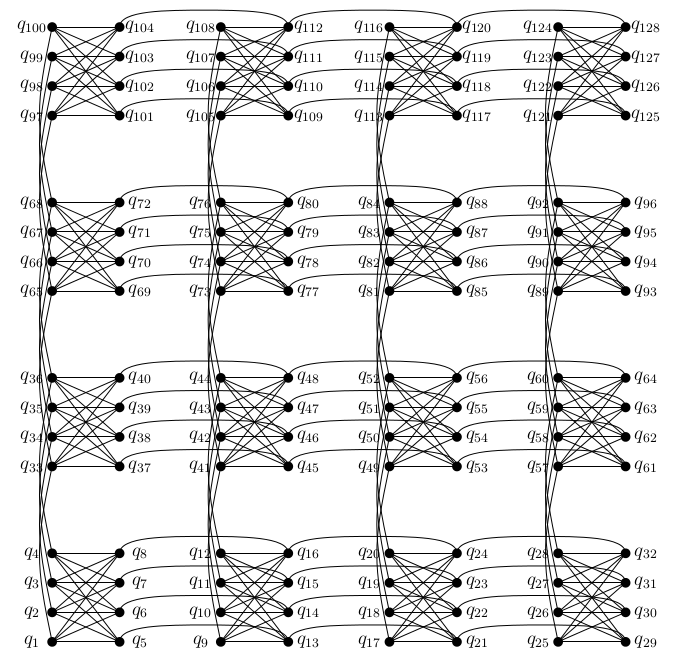
\includegraphics[width=\linewidth/2]{resources/images/chimera.png}}
  \caption{16 Chimera cells, called a $C4$}
  \label{fig:boat1}
\end{figure}

Though there are many parameters that the D-Wave chip accepts, the main process of using it to solve problems is to send a problem $h$ and $J$, and then receive a number of ``reads" back that are the solutions the chip found.

\section{Graph Embedding}

The fixed shape of the Chimera graph of the D-Wave annealer introduces the problem of running graphs with non-Chimera topologies. Obviously not all interesting Ising problems can be simply placed onto a Chimera graph using a single qubit for every problem variable and single coupler for every problem edge. For instance, I wanted to find the best ways of running 3D lattice Ising problems on the D-Wave processor.

To get around this, we use several qubits and their couplers to form a \textit{chain} which then represents a single variable from the original problem. If we assign a \textit{chain weight} to the couplers of the chain of low enough negative value relative the rest of the weights in the problem $J$, the chain should always align itself such that all of its qubits have the same spin. If we can find a set of chains on the Chimera graph corresponding to problem variables such that if there is an edge between two problem variables there is also a coupler in the Chimera graph between at least one pair of qubits in each chain, then we have found an embedding of the problem graph for the Chimera.

To make this more formal, for an embedding of a graph $G$ with $n$ vertices $V_G = \{v_1, v_2, \ldots, v_n\}$ on graph $H$ with $m$ vertices $V_H = \{u_1, u_2, \ldots, u_m\}$, we define an embedding $M: v_i \in V_G \rightarrow \mathbf{s}_i \subset V_G$. For $M$ to be a valid embedding, there are three requirements:
\begin{enumerate}
	\item All $\mathbf{s}_i$ must be disjoint with each other, i.e. for all $1 \leq i < j \leq n$, $\mathbf{s}_i \cap \mathbf{s}_j = \emptyset$.
	\item All $\mathbf{s}_i$ must be connected in $H$. This means that for all $u_j \in \mathbf{s}_i$, there is at least one other vertex $u_k \in \mathbf{s}_i$ such that $u_ju_k \in E(H)$.
	\item If there is an edge $v_iv_j \in E(G)$, then there are some $u_{i*}$ and $u_{j*}$ such that $u_{i*}u_{j*} \in E(H)$. This ensures that for any edge in $G$, there is at least one corresponding edge in $H$ that we can map to.
\end{enumerate}

For an example, let's take a $K_3$ complete graph (called $G$ with vertices $1,2,3$) and embed it in a $C_5$ cyclic graph with 5 vertices (called $H$ with vertices $a,b,c,d,e$).

\centerline{
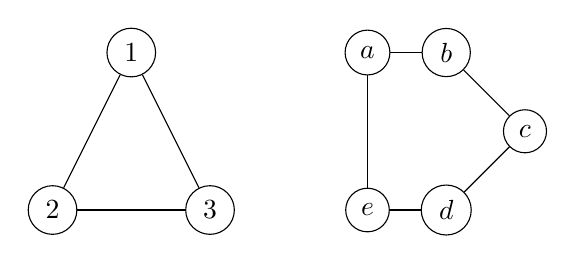
\begin{tikzpicture}
	\draw (1,2) node(g1) [draw, circle] {$1$};
	\draw (0,0) node(g2) [draw,circle] {$2$};
	\draw (2,0) node(g3) [draw,circle] {$3$};	
	\draw (4,2) node(ha) [draw,circle] {$a$};
	\draw (5,2) node(hb) [draw, circle] {$b$};
	\draw (6,1) node(hc) [draw, circle] {$c$};
	\draw (5,0) node(hd) [draw, circle] {$d$};
	\draw (4,0) node(he) [draw, circle] {$e$};
	\path[draw] (g1) -- (g2);
	\path[draw] (g2) -- (g3);
	\path[draw] (g3) -- (g1);
	\path[draw] (ha) -- (hb);
	\path[draw] (hb) -- (hc);
	\path[draw] (hc) -- (hd);
	\path[draw] (hd) -- (he);
	\path[draw] (he) -- (ha);
\end{tikzpicture}}

Now we can create an embedding by noticing that we can group $b$ and $c$ together and $e$ and $d$ in $H$ to get the same graph as $G$. Let $M$ be our embedding and let

$$M(1) \rightarrow \{a\}$$
$$M(2) \rightarrow \{e,d\}$$
$$M(3) \rightarrow \{b,c\}$$

$M$ is a valid embedding because the sets of vertices in $H$ it produces are disjoint, the sets are connected, and because each edge in $G$ can be mapped to at least one edge in $H$ ($12 \rightarrow ae$, $23 \rightarrow dc$, and $13 \rightarrow ab$).

Most of the time, there is not a single way to embed a given graph onto another (in the example, we could have mapped $1 \rightarrow \{a,b,c\}$ and still gotten a valid embedding). When embedding an Ising problem on the D-Wave hardware, how the embedding is done affects the performance of the hardware on the original problem. Several factors such as average chain length, how different the chain lengths are in the embedding, how symmetric the chains are, chain strength, and the number of available couplers between chains, all affect how easily the hardware is able to find good solutions to the original problem.

\subsection{Algebraic Chain Strength}

The algebraic chain strengths of the chains in an embedding for a given problem $h$ and $J$ is defined as the minimum absolute value that we can assign to the weight of the edges of the chains such that every ground state of the embedded problem corresponds to a ground state of the original (or \textit{logical}) problem. This is equivalent to stating that every ground state of the embedded problem will have no \textit{broken chains}, or chains where some of the qubits are spin up and the others are spin down. There is a simple way to calculate the algebraic chain strength. For each edge in the chain, calculate the sum of the absolute values of the edge weights coming off the entire chain on side of the edge, and then on the other side. The algebraic chain strength is the minimum of two values.

Consider an example: a chain of 4 qubits $q_0, q_1, q_2, q_3$ such that there is chain edge from $q_0$ to $q_1$, $q_1$ to $q_2$, and $q_2$ to $q_3$. Each of these qubits has single edge coming off of it representing an original problem edge. Now examine the edge in the middle, $q_1q_2$. On one side, there are two qubits $q_0, q_1$ for which the sum of the absolute values of the logical edges is 6. On the other side, qubits $q_2, q_3$ have a sum of the absolute edge weights of 3. Thus the algebraic chain strength for this chain is $min(6,3) = 3$.

\centerline{
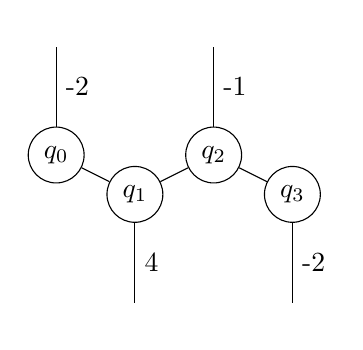
\begin{tikzpicture}
	\draw (1,1.5) node(v1) [draw,circle] {$q_0$};
	\draw (2,1) node(v3) [draw,circle] {$q_1$};
	\draw (3,1.5) node(v4) [draw,circle] {$q_2$};
	\draw (4,1) node(v2) [draw,circle] {$q_3$};
	\draw (1,3) node(v104) {};
	\draw (2,-0.5) node(v105) {};
	\draw (3,3) node(v106) {};
	\draw (4,-0.5) node(v107) {};
	\path[draw] (v2) -- (v4);
	\path[draw] (v1) -- (v3);
	\path[draw] (v3) -- (v4);
	\path[draw] (v1) -- node [right] {-2} (v104);
	\path[draw] (v3) -- node [right] {4} (v105);
	\path[draw] (v4) -- node [right] {-1} (v106);
	\path[draw] (v2) -- node [right] {-2} (v107);
\end{tikzpicture}}

\section{Embedding 3D Lattice Ising Problems}

Physicists are interested in 3D lattice Ising problems, where the problem graph is a 3D grid. This means every variable in paired with 6 others, or 2 each in the $x$, $y$ and $z$ directions. I looked at two subsets of these problems: $4*k*k$ lattices and $8*k*k$ lattices. 

For $4*k*k$ lattices, there is a simple embedding for the Chimera graph where every chain has two qubits. Thus each Chimera tile (a $K_{4,4}$) has a $4*1*1$ column of the original problem lattice embedded in it. All of the chains are symmetric with an algebraic chain strength of 3. The vertical $z$-axis edges of the column were all contained within a single tile, and then the $x$ and $y$-axis edges became the couplers going between tiles. Since there is a single obvious way to do this embedding, I did not spend much time on it.

For $8*k*k$ lattices, the best embeddings use chains of 4 qubits. A single $8*1*1$ column of the lattice is embedding into a square of 4 Chimera tiles, called a $C2$ (note a $C2$ has $4\cdot8=32$ total qubits, allowing 8 chains of 4 qubits each). In each of the embeddings, the chains take the same shape, and the $x$ and $y$-axis edges become the couplers connecting $C2$'s together. The only differences were in the placement of the $z$-axis edges, which could either be connected to the two qubits on either end of the chain, or to the two qubits in the middle of the chain. For each of these possible embeddings, it is also possible to ``split" the $z$-axis edge and put it on two couplers, as each chain is connected two every other with two couplers. Instead of putting the full weight of the original lattice edge, we use $1/2$ the original weight on each coupler. In total, this allowed for 4 embeddings. I worked primarily on testing which of these embeddings produced the best results.

\textbf{Note:} In the following diagrams, the left side has a C4 ($4*4$ Chimera cells) with a $8*4*4$ lattice embedded on it, where blue couplers belong to a chain, and red edges go between chains corresponding to the original lattice edges. On the right, a single chain is shown with a similar color scheme ($z$-axis couplers are highlighted with green as they are the only edges that change among the embeddings).

\begin{figure}[h!]
  \centerline{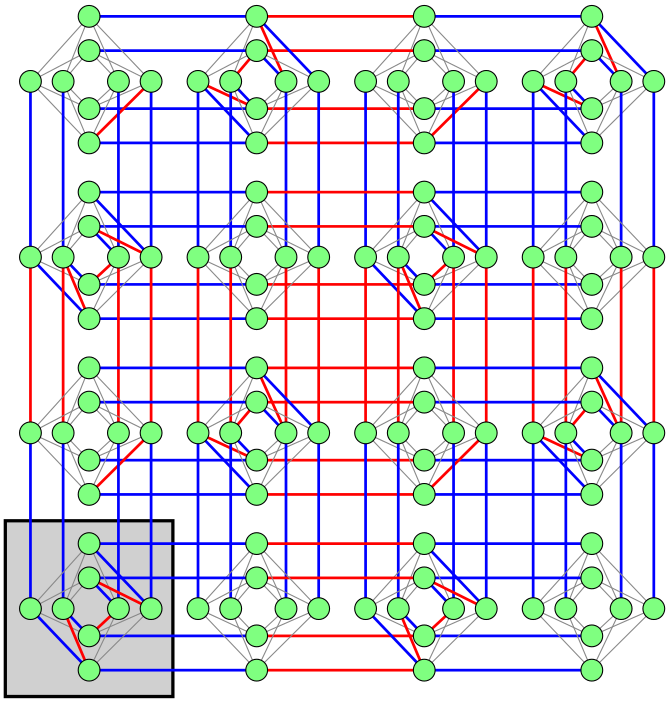
\includegraphics[width=\linewidth/3]{resources/images/emb1.png}\hspace{1cm}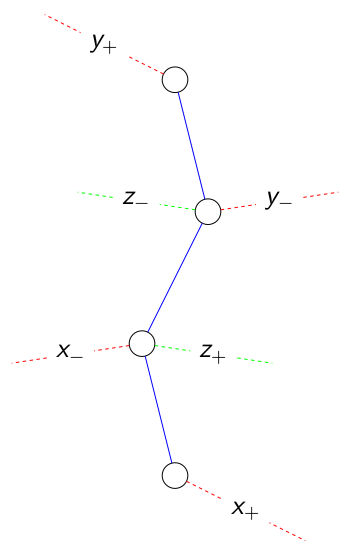
\includegraphics[height=\linewidth/3]{resources/images/emb1_chain.png}}
  \caption{\textbf{Left:} Embedding 1. A C4 with the first embedding I did. The C4 embeds a $8*2*2$ lattice. \textbf{Right:} A single chain diagram for this embedding.}
  \label{fig:boat1}
\end{figure}

\begin{figure}[h!]
  \centerline{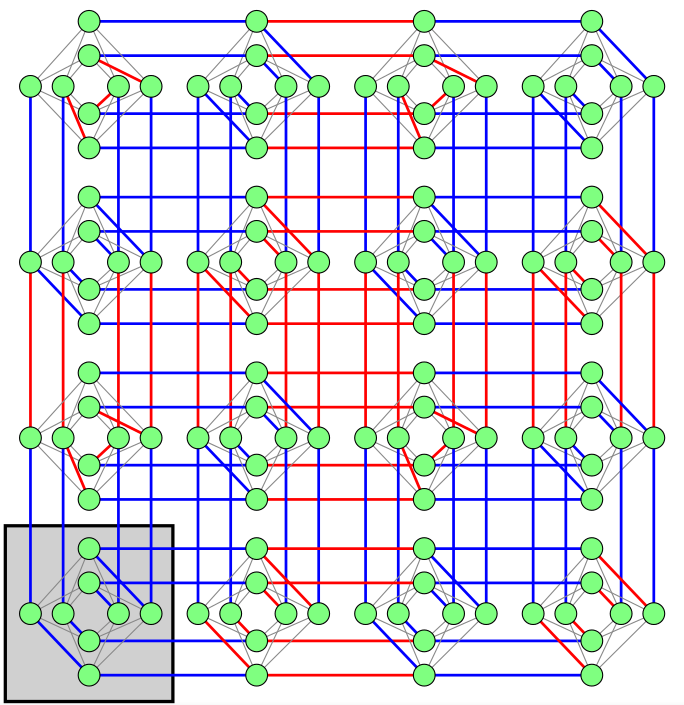
\includegraphics[width=\linewidth/3]{resources/images/emb2.png}\hspace{1cm}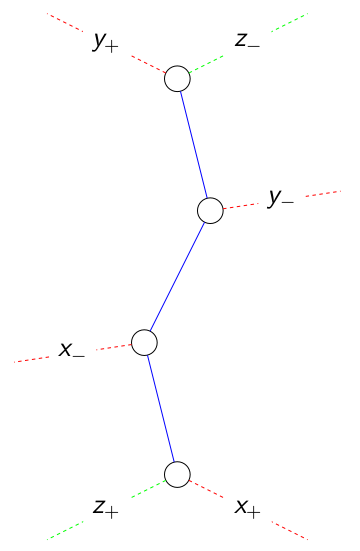
\includegraphics[height=\linewidth/3]{resources/images/emb2_chain.png}}
  \caption{\textbf{Left:} Embedding 2. Instead of placing $z$-axis edges on the middle of the chain, they were placed on the end. \textbf{Right:} A single chain diagram for this embedding.}
  \label{fig:boat1}
\end{figure}

\begin{figure}[h!]
  \centerline{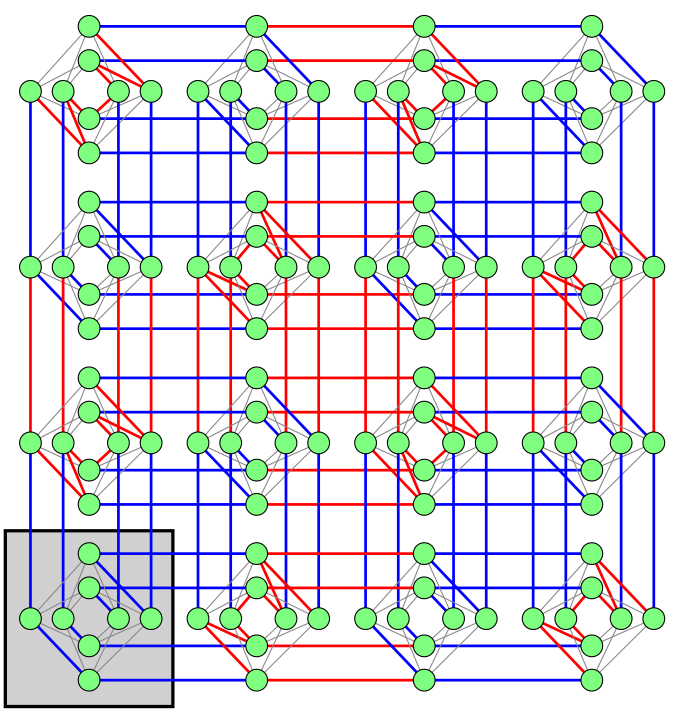
\includegraphics[width=\linewidth/3]{resources/images/emb3.png}\hspace{1cm}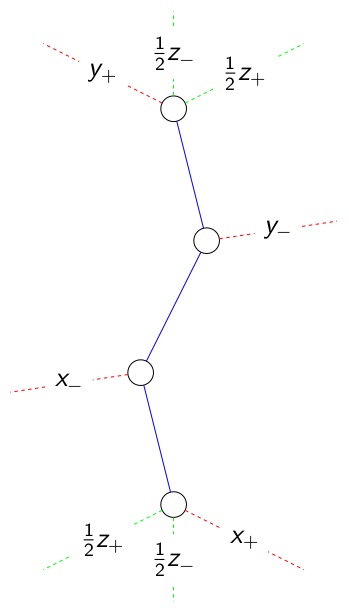
\includegraphics[height=\linewidth/3]{resources/images/emb3_chain.png}}
  \caption{\textbf{Left:} Embedding 3. Similar to embedding 2, but the $z$-axis edges are spread across the two available couplers. \textbf{Right:} A single chain diagram for this embedding. Note that this will reduce the algebraic chain strength to 2 instead of 3 as with embedding 2.}
  \label{fig:boat1}
\end{figure}

\begin{figure}[h!]
  \centerline{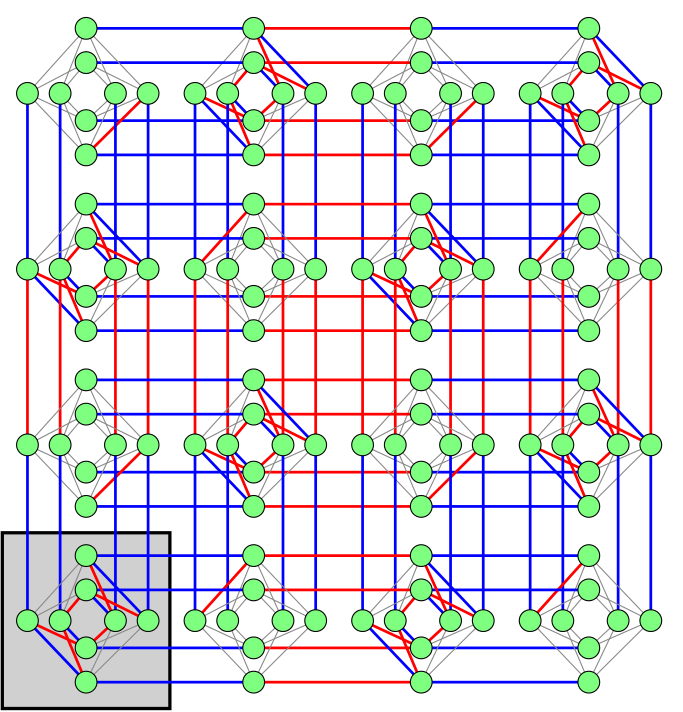
\includegraphics[width=\linewidth/3]{resources/images/emb4.png}\hspace{1cm}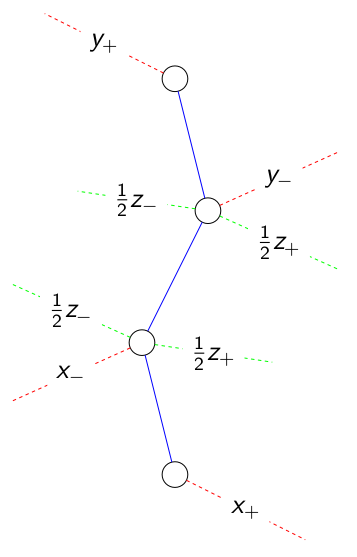
\includegraphics[height=\linewidth/3]{resources/images/emb4_chain.png}}
  \caption{\textbf{Left:} Embedding 4. Similar to embedding 1, but with split $z$-axis edges. \textbf{Right:} A single chain diagram for this embedding. Again, the algebraic chain strength has been reduced to 2 from 3.}
  \label{fig:boat1}
\end{figure}

\vspace{10cm}
\subsection{Chain Strength}

Apart from testing the four embeddings, another important factor was determining the best chain strength to use for a given embedding. Though it would be ideal to set the chain strength to be the algebraic chain strength or greater of each embedding, this does not always give the best results. This is because the D-Wave processor has a limited energy scale available, and the energy scale is quantized and not perfectly accurate. This means as we increase the chain strength, the weights of the problem edges must go down and will eventually be distorted.

\section{Success Statistics}
Several different important statistics were used to measure the success an embedding. These were useful in comparing the embeddings and deciding which was best.

\begin{enumerate}
\item\textbf{Success probability}

This is simply a measure of how likely the D-Wave chip would find a ground state of the original problem. However, as the problems got bigger and bigger, it became infeasible to get enough reads from the chip to accurately determine the success probability. Thus other statistics were also used.

\item\textbf{Mean residual energy}

A certain state's residual energy is the difference between the energy of the state and the ground energy of the problem. Thus the mean residual energy for a collection of solutions returned is the mean of the residual energies of the states. Though this will give a good indication of how well a technique is at solving some problems, it is still possible to have a low mean residual energy while still having a low success probability (as there may be many easy low energy states but hard to reach ground states).

\item\textbf{Broken chain probability}

The probability that a chain would be broken for a given read. This is also a good indicator of how well an embedding is performing, but if using a post processing technique as mentioned before, it does not directly correlated to success probability or mean residual energy. It is quite possible to have an embedding and chain strength that results in more broken chains but higher success probability, etc.

\item\textbf{Time to solution}

Time to solution is a success statistic based on the amount of ``time", or in the case of the D-Wave machine the number of reads, needed such that there is a 99\% chance of achieving a ground state. The time to solution $t$ for a success probability $s$ is
$$(1-s)^t < 0.01$$
$$t\cdot \log(1-s) < \log(0.01)$$
$$t > \frac{\log(0.01)}{\log(1-s)}$$

If we want to compare techniques which have different computation times (as opposed to just using a ``read" as a single unit of time), such as with simulated annealing where the computation time is based on the number of sweeps, we can multiply this final value by that time. 
\end{enumerate}

By examining these statistics across the four embeddings as well as a variety of chain strengths on random problems, I was able to determine the best embedding and chain strength for use on the D-Wave processor. I also compared the performance of the D-Wave processor against simulated annealing both on the original lattice problems as well as the embedded problems. Since simulated annealing gives a good approximation for how hard a problem is, these served as benchmarks for the D-Wave processor.

\chapter{Conclusion}

Despite quantum computing only offering a speedup for a limited class of problems, it still offers endless possible applications. In this Keystone I have discussed algorithms that can search a problem space efficiently, perform an associative memory recall, run the discrete Fourier transform, and solve graph problems with applications in physics. However, quantum computing as a field still faces many challenges that it must overcome to be truly useful outside of academia.

One of the most prominent of these is the physical construction of the computers. D-Wave's accomplishments on the front of quantum annealing, such as their 2048-qubit annealer, are impressive, but it remains difficult to classify their performance. However, recent iterations appear to be beating out the classical solvers on hard Ising problems by large factors \cite{googleblog}. For universal or gate based quantum computers, which are necessary for the more famous algorithms such as Grover's and Shor's, progress is slow. 21 remains the largest number factored on a quantum computer using Shor's algorithm \cite{martinlopez}. Scalable gate-based designs remain out of reach.

Another problem faced by quantum computing is that it remains difficult to access for those who are not physicists. If it is to have a large impact, quantum computing will need to be accessible to programmers and people without a physics background. This means a large amount of work will need to be put into developing tooling and better educational resources such that people can start writing applications for these new computers. In the future, I hope to work on creating these resources, and ideally, contribute to the expanding area of quantum computing research. 


\begin{thebibliography}{9}
\addcontentsline{toc}{chapter}{Bibliography}
\raggedright
  
  \bibitem{apps14}
  “Applications: Helping solve some of the most difficult challenges.” (2014). Retrieved from http://www.dwavesys.com/quantum-computing/applications
  
  \bibitem{ein05}
  Einstein, A. (1905). Über einen die Erzeugung und Verwandlung des Lichtes betreffenden heuristischen Gesichtspunkt. Annalen der Physik, 322(6), 132-148.

  \bibitem{grover96}
  Grover, L. K. (1996). A fast quantum mechanical algorithm for database search. \emph{In Proceedings of the twenty-eighth annual ACM symposium on Theory of computing} (pp. 212-219). ACM.

  \bibitem{kothari12}
  Kothari, R. (2012). How much does a quantum oracle to find a needle in a haystack really cost? Retrieved January 20, 2017, from http://mathoverflow.net/questions/102779/how-much-does-a-quantum-oracle-to-find-a-needle-in-a-haystack-really-cost

  \bibitem{martinlopez}
  Martín-López, E., Laing, A., Lawson, T., Alvarez, R., Zhou, X. Q., \& O'brien, J. L. (2012). Experimental realization of Shor's quantum factoring algorithm using qubit recycling. \emph{Nature Photonics}, 6(11), 773-776.

  \bibitem{meh01}
  Mehra, J., \& Rechenberg, H. (2001). The historical development of quantum theory (Vol. 1). \emph{Springer Science \& Business Media}.
  
  \bibitem{mer07}
  Mermin, N. D. (2007). \emph{Quantum Computer Science: An Introduction}. New York, NY: Cambridge University Press.

  \bibitem{Kha15}
  Moammer, K. (2015). Intel Abandoning Silicon With 7nm and Beyond - Silicon Alternatives Coming By 2020. \emph{Wccf tech}. Retrieved from http://wccftech.com/intel-abandoning-silicon-7nm/

  \bibitem{moo65}
  Moore, G.E. (1965). Cramming More Components Onto Integrated Circuits. Electronics, 38(8), 82-85.

  \bibitem{nev13}
  Neven, H. (2013). Launching the Quantum Artificial Intelligence Lab. Retrieved from http://googleresearch.blogspot.ca/2013/05/launching-quantum-artificial.html
  
  \bibitem{googleblog}
  Neven, H. (2015). When can Quantum Annealing win? Retrieved from https://research.googleblog.com/2015/12/when-can-quantum-annealing-win.html  
  
  \bibitem{dwa14}
  “Quantum Computing: How D-Wave Systems Work.” (2014). Retrieved from http://www.dwavesys.com/quantum-computing
  
  \bibitem{rojas04}
  Rojas, R. (2004). A tutorial introduction to the lambda calculus. Retrieved from http://www.utdallas.edu/\textasciitilde gupta/courses/apl/lambda.pdf.  
  
  \bibitem{schr26}
  Schrödinger, E. (1926). An undulatory theory of the mechanics of atoms and molecules. Physical Review, 28(6), 1049.

  \bibitem{Sim16}
  Simonite, T. (2016). Intel Puts the Brakes on Moore's Law. \emph{MIT Technology Review}. Retrieved from https://www.technologyreview.com/s/601102/intel-puts-the-brakes-on-moores-law/

   \bibitem{smi15}
   Smith, B. (n.d.). ``Quantum Ideas: Week 2" Lecture Notes. \emph{University of Oxford}. Retrieved from https://users.physics.ox.ac.uk/~smithb/website/coursenotes/qi/QILectureNotes2.pdf

  \bibitem{spector04}
  Spector, L. (2004). Automatic Quantum Computer Programming: a genetic programming approach (Vol. 7). \emph{Springer Science and Business Media}.

  \bibitem{tonder04}
  Van Tonder, A. (2004). A lambda calculus for quantum computation. \emph{SIAM Journal on Computing}, 33(5), 1109-1135.

  \bibitem{Ven00}
  Ventura, D., \& Martinez, T. (2000). Quantum associative memory. \emph{Information Sciences}, 124(1), 273-296.

  \bibitem{foldit}
  What is protein folding? (n.d.). \emph{Foldit}. Retrieved January 20, 2017, from http://fold.it/portal/info/about

\end{thebibliography}

\begin{appendix}
	\chapter{quantum-computer-simulator.rkt}
	\begin{lstlisting}
#lang racket
(require math)
(require racket/vector)

(require srfi/1)
(require 2htdp/batch-io)
(define-namespace-anchor a)
(define ns (namespace-anchor->namespace a))

(provide matrix-print initialize-register measure-register apply-gate)
(provide register Hadamard-gate Pauli-X-gate Pauli-Y-gate Pauli-Z-gate CNOT-gate QSwap-gate Toffoli-gate)
(provide bits bits->row-matrix set-register) ; for Grover.rkt
(provide G-nqubit-constructor) ; for oracle-constructor.rkt

;--------------------Quantum simulator functions---------------------;

(define matrix-print (lambda (matrix)
	(let ([size (square-matrix-size matrix)])
		(for ([m size]) (for ([n size])
				(display (array-ref matrix (list->vector (list m n)))) (display " "))
			(displayln "")))))

(define bits (lambda (n l) ; Returns a list length l of the digits of n in binary with leading zeroes
	(let ([n-bits null])
		(set! n-bits (let loop ((n n) (binary '()))
			(if (= 0 n) 
				binary
				(loop (arithmetic-shift n -1) (cons (bitwise-and n 1) binary)))))
		(append (build-list (- l (length n-bits)) (lambda (x) 0)) n-bits))))

(define bits->dec (lambda (n)
	(string->number (string-append "#b" (foldr string-append "" (map number->string n))))))

(define bits->row-matrix (lambda (bits)
	(build-matrix 1 (length bits) (lambda (i j) (list-ref bits j)))))

(define register null)

(define set-register (lambda (psi)
	(set! register psi)))

(define initialize-register (lambda (lq)
	(set! register (array->mutable-array (make-array (list->vector (list 1 (expt 2 (length lq)))) 0)))
	(array-set! register (list->vector (list 0 (bits->dec lq))) 1)
	(set! register (mutable-array-copy register))))

(define measure-register (lambda ()
	(let ([psi (matrix->list register)] [q-index 0] [max 0] [probabilities null])
		(set! probabilities (map (lambda (qubit) (magnitude qubit)) psi))
		(for ([qubit (length psi)])
			(when (< max (list-ref probabilities qubit))
				(set! max (list-ref probabilities qubit))
				(set! q-index qubit)))
		(display "The most likely result is |") 
		(display (~r q-index #:base 2 #:min-width (exact-round (/ (log (length psi)) (log 2))) #:pad-string "0"))
		(display "> with a probability of ") (displayln (* max max)))))

(define G-nqubit-constructor (lambda (N Q G)
	(let ([Q (reverse Q)] [n (exact-round (/ (log N) (log 2)))] [i-binary '()] [j-binary '()] [i-j-differ #f] [Qprime '()] [i-star '()] [j-star '()])
		(set! Qprime (for/list ([index n] #:when (not (member index Q))) index))
		(build-matrix N N (lambda (i j)
			(letrec
				([i-binary (bits i n)] 
				[j-binary (bits j n)] 
				[i-j-checker (lambda (Qprime)
					(cond [(null? Qprime) 
							(array-ref G (list->vector (map bits->dec (map reverse (call-with-values 
								(lambda () (for/lists (l1 l2) ([x Q]) (values 
									(list-ref i-binary x) 
									(list-ref j-binary x)))) list)))))]
						[(not (= (list-ref i-binary (car Qprime)) (list-ref j-binary (car Qprime)))) 0]
						[else (i-j-checker (cdr Qprime))]))])
				(i-j-checker Qprime)))))))

(define apply-gate (lambda (psi qubits G)
	(let ([new-psi (matrix* psi (G-nqubit-constructor (matrix-num-cols register) qubits G))])
		(set! register new-psi)
		new-psi)))

;----------------Quantum gates--------------------;

(define 1oversqrt2 (/ 1 (sqrt 2)))

(define Hadamard-gate (matrix [
	[1oversqrt2 1oversqrt2]
	[1oversqrt2 (* 1oversqrt2 -1)]
]))

(define Pauli-X-gate (matrix [ ; also known as the NOT gate
	[0 1]
	[1 0]
]))

(define Pauli-Y-gate (matrix [
	[0 0-i]
	[0+i 0]
]))

(define Pauli-Z-gate (matrix [
	[1 0]
	[0 -1]
]))

(define CNOT-gate (matrix [
	[1 0 0 0]
	[0 1 0 0]
	[0 0 0 1]
	[0 0 1 0]
]))

(define QSwap-gate (matrix [
	[1 0 0 0]
	[0 0 1 0]
	[0 1 0 0]
	[0 0 0 1]
]))

(define Toffoli-gate (matrix [ ; also known as the CCNOT gate
	[1 0 0 0 0 0 0 0]
	[0 1 0 0 0 0 0 0]
	[0 0 1 0 0 0 0 0]
	[0 0 0 1 0 0 0 0]
	[0 0 0 0 1 0 0 0]
	[0 0 0 0 0 1 0 0]
	[0 0 0 0 0 0 0 1]
	[0 0 0 0 0 0 1 0]
]))
	\end{lstlisting}
	\chapter{grover.rkt}
	\begin{lstlisting}
#lang racket
(require math)
(require racket/vector)

(require srfi/1)
(require 2htdp/batch-io)
(define-namespace-anchor a)
(define ns (namespace-anchor->namespace a))

(require "quantum-computer-simulator.rkt")

(provide generate-fake-Oracle Grover)
(provide phase-flip-0-state) ; for oracle-constructor.rkt

;-----------Constructors for the gates for Grover's algorithm--------;

(define make-Hadamard (lambda (N)
	(let ([constant (exact->inexact (/ 1 (expt 2 (/ (/ (log N) (log 2)) 2))))])
		(build-matrix N N (lambda (i j)
			(* constant (expt -1 (matrix-dot (bits->row-matrix (bits i N)) (bits->row-matrix (bits j N))))))))))

(define H-matrix null)

(define Hadamard (lambda (psi)
	(cond
		[(or (null? H-matrix) (not (eq? (matrix-num-cols H-matrix) (matrix-num-cols register))))
			(set! H-matrix (make-Hadamard (matrix-num-cols register)))
			(let ([new-psi (matrix* psi H-matrix)])
				(set-register new-psi)
				new-psi)]
		[else (let ([new-psi (matrix* psi H-matrix)])
			(set-register new-psi)
			new-psi)])))

(define pf-matrix null)

(define make-phase-flipper (lambda (N)
	(diagonal-matrix (cons -1 (build-list (sub1 (matrix-num-cols register)) (lambda (x) 1))))))

(define phase-flip-0-state (lambda (psi)
	(cond
		[(or (null? pf-matrix) (not (eq? (matrix-num-cols pf-matrix) (matrix-num-cols register))))
			(set! pf-matrix (make-phase-flipper (matrix-num-cols register)))
			(let ([new-psi (matrix* psi pf-matrix)])
				(set-register new-psi)
				new-psi)]
		[else (let ([new-psi (matrix* psi pf-matrix)])
			(set-register new-psi)
			new-psi)])))

(define U_omega null)

(define Oracle (lambda (psi)
	(let ([new-psi (matrix* psi U_omega)])
		(set-register new-psi)
		new-psi)))

(define generate-fake-Oracle (lambda (N solution)
	(diagonal-matrix (append (build-list solution (lambda (x) 1)) '(-1) (build-list (sub1 (- N solution)) (lambda (x) 1))))))

(define Grover (lambda (input-U_omega) ; An implementation of Grover's algorithm, input-U_omega is a matrix representation the oracle operator
	(let ([steps 0] [qubits (exact-round (/ (log (matrix-num-cols input-U_omega)) (log 2)))]) ; Requires log(N) qubits where N is the width of the matrix representing U_omega
		(cond
			[(= qubits 1) (set! steps 0)]
			[(= qubits 2) (set! steps 1)]
			[else (set! steps (exact-round (* (/ pi 4) (sqrt (expt 2 qubits)))))]) ; # of steps ~pi*sqrt(N)/4

		(set! U_omega input-U_omega)
		(display "The number of required qubits is ") (displayln qubits)
		(display "Number of operations required is ") (displayln (+ 1 steps))

		(initialize-register (build-list qubits (lambda (x) 0)))	; Initialize all qubits to |0>

		(Hadamard register)	; Apply a Hadamard gate to all qubits

		(for ([i steps])
			(Hadamard (phase-flip-0-state (Hadamard (Oracle register))))) ; Apply the Grover Diffusion operator
		)))
	\end{lstlisting}
	\chapter{oracle-constructor.rkt}
	\begin{lstlisting}
#lang racket
(require math)
(require racket/vector)

(require srfi/1)
(require 2htdp/batch-io)
(define-namespace-anchor a)
(define ns (namespace-anchor->namespace a))

(require "quantum-computer-simulator.rkt")
(require "Grover.rkt")

(provide NOT NOT OR OR AND AND Grover-from-classical-circuit U_omega input-qubits generate-U_omega)

;--------------

(define Oracle (lambda (psi)
	(matrix* psi U_omega)))

(define total-qubits 0)

(define next-safe-qubit 0)

(define uncomputer null)

(define computer-strings-for-latex "")
(define uncomputer-strings-for-latex "")

(define Pauli-X (lambda (n qubit)
	(G-nqubit-constructor (expt 2 n) (list qubit) Pauli-X-gate)))

(define Toffoli (lambda (n qubits)
	(G-nqubit-constructor (expt 2 n) qubits Toffoli-gate)))

(define NOT (lambda (qubit)
	(set! computer-strings-for-latex (string-append computer-strings-for-latex (string-append "\tX\tq" (number->string qubit) "\n"))) ; just for LaTeX output
	(set! U_omega (matrix* U_omega (Pauli-X total-qubits qubit)))
	(set! uncomputer (matrix* (Pauli-X total-qubits qubit) uncomputer))
	(set! uncomputer-strings-for-latex (string-append (string-append "\tX\tq" (number->string qubit) "\n") uncomputer-strings-for-latex)) ; just for LaTeX output
	qubit))

(define OR (lambda (qubit1 qubit2)
	(void (NOT qubit1))
	(void (NOT qubit2))
	(set! U_omega (matrix* U_omega (Toffoli total-qubits (list qubit1 qubit2 next-safe-qubit))))
	(set! computer-strings-for-latex (string-append computer-strings-for-latex (string-append "\ttoffoli\tq" (number->string qubit1) ",q" (number->string qubit2) ",q" (number->string next-safe-qubit) "\n"))) ; just for LaTeX output
	(set! uncomputer (matrix* (Toffoli total-qubits (list qubit1 qubit2 next-safe-qubit)) uncomputer))
	(set! uncomputer-strings-for-latex (string-append (string-append "\ttoffoli\tq" (number->string qubit1) ",q" (number->string qubit2) ",q" (number->string next-safe-qubit) "\n") uncomputer-strings-for-latex)) ; just for LaTeX output
	(void (NOT qubit1))
	(void (NOT qubit2))
	(void (NOT next-safe-qubit))
	(set! next-safe-qubit (+ next-safe-qubit 1))
	(- next-safe-qubit 1))) ; This, by defintion, is the output of the toffoli gate (the third qubit), so that's what we want to return

(define AND (lambda (qubit1 qubit2)
	(set! U_omega (matrix* U_omega (Toffoli total-qubits (list qubit1 qubit2 next-safe-qubit))))
	(set! computer-strings-for-latex (string-append computer-strings-for-latex (string-append "\ttoffoli\tq" (number->string qubit1) ",q" (number->string qubit2) ",q" (number->string next-safe-qubit) "\n"))) ; just for LaTeX output
	(set! uncomputer (matrix* (Toffoli total-qubits (list qubit1 qubit2 next-safe-qubit)) uncomputer))
	(set! uncomputer-strings-for-latex (string-append (string-append "\ttoffoli\tq" (number->string qubit1) ",q" (number->string qubit2) ",q" (number->string next-safe-qubit) "\n") uncomputer-strings-for-latex)) ; just for LaTeX output
	(set! next-safe-qubit (+ next-safe-qubit 1))
	(- next-safe-qubit 1))) ; This, by defintion, is the output of the toffoli gate (the third qubit), so that's what we want to return

(define get-extra-qubits (lambda (boolean-expression)
	(cond
		[(null? boolean-expression) 0]
		[(or (eq? 'OR (car boolean-expression)) (eq? 'AND (car boolean-expression))) (+ 1 (get-extra-qubits (cdr boolean-expression)))]
		[(list? (car boolean-expression)) (+ (get-extra-qubits (car boolean-expression)) (get-extra-qubits (cdr boolean-expression)))]
		[else (get-extra-qubits (cdr boolean-expression))])))

(define get-base-qubits (lambda (boolean-expression)
	(cond
		[(null? boolean-expression) 0]
		[(number? (car boolean-expression)) (max (car boolean-expression) (get-base-qubits (cdr boolean-expression)))]
		[(list? (car boolean-expression)) (max (get-base-qubits (car boolean-expression)) (get-base-qubits (cdr boolean-expression)))]
		[else (get-base-qubits (cdr boolean-expression))])))

(define controlled-Z-gate (matrix [
	[1 0 0 0]
	[0 1 0 0]
	[0 0 1 0]
	[0 0 0 -1]
]))

(define U_omega null)

(define input-qubits null)

(define generate-U_omega (lambda (boolean-expression)
	(let ([base-qubits (+ 1 (get-base-qubits boolean-expression))] [temp-matrix '()]) ; base-qubits is equal to the # of qubits needed to implement the circuit before uncomputation
		(set! input-qubits (- base-qubits 1))
		(set! next-safe-qubit base-qubits)
		(set! total-qubits (+ base-qubits (get-extra-qubits boolean-expression) 2)) ; Two extra: one to save the answer before we uncompute, and another for the phase flipper
		(set! U_omega (identity-matrix (expt 2 total-qubits)))
		(set! uncomputer (identity-matrix (expt 2 total-qubits)))
		(eval boolean-expression ns)
		(set! U_omega (matrix* U_omega (G-nqubit-constructor (expt 2 total-qubits) (list (- total-qubits 3) (- total-qubits 2)) CNOT-gate))) ; Copy output of simulated classical circuit to the nth qubit
		(set! U_omega (matrix* U_omega uncomputer))
		(set! U_omega (matrix* U_omega 
			(G-nqubit-constructor (expt 2 total-qubits) (list (- total-qubits 2) (- total-qubits 1)) CNOT-gate)
			(G-nqubit-constructor (expt 2 total-qubits) (list (- total-qubits 2) (- total-qubits 1)) controlled-Z-gate)
			(G-nqubit-constructor (expt 2 total-qubits) (list (- total-qubits 2) (- total-qubits 1)) CNOT-gate)
			U_omega))
		(void (write-file "./circuit-files/qcircuit.qasm" (string-append
			"\tqubit\tq" (string-join (map (lambda (num) (number->string num)) (range total-qubits)) ",0\n\tqubit\tq") ",0\n" ; Set up necessary qubits
			computer-strings-for-latex ; Add the compute string
			"\tcnot\tq" (number->string (- total-qubits 3)) ",q" (number->string (- total-qubits 2)) "\n" ; CNOT for the copy on to (n-1)th qubit
			uncomputer-strings-for-latex ; Add the uncompute string
			"\tcnot\tq" (number->string (- total-qubits 2)) ",q" (number->string (- total-qubits 1)) "\n" ; CNOT for the copy on to nth qubit
			"\tc-z\tq" (number->string (- total-qubits 2)) ",q" (number->string (- total-qubits 1)) "\n" ; controlled Z on (n-1)th and nth qubits
			"\tcnot\tq" (number->string (- total-qubits 2)) ",q" (number->string (- total-qubits 1)) "\n" ; CNOT for the uncopy on to nth qubit
			computer-strings-for-latex ; Now we do the whole first half again, starting with the compute string
			"\tcnot\tq" (number->string (- total-qubits 3)) ",q" (number->string (- total-qubits 2)) "\n" ; CNOT for the uncopy on to (n-1)th qubit
			uncomputer-strings-for-latex ; Add the uncompute string
		))))))

(define special-make-Hadamard (lambda (N up-to-qubit)
	(letrec ([apply-H (lambda (M qubit)
		(cond
			[(= qubit up-to-qubit) (matrix* M (G-nqubit-constructor N (list qubit) Hadamard-gate))]
			[else (matrix* M (apply-H (G-nqubit-constructor N (list qubit) Hadamard-gate) (+ qubit 1)))]))])
		(apply-H (identity-matrix N) 0))))

(define Grover-from-classical-circuit (lambda (input-U_omega input-qubits) ; An implementation of Grover's algorithm, input-U_omega is a matrix representation the oracle operator
	(let ([special-Hadamard null]
		[special-H-matrix (special-make-Hadamard (matrix-num-cols input-U_omega) input-qubits)] 
		[steps 0] 
		[qubits (exact-round (/ (log (matrix-num-cols input-U_omega)) (log 2)))]) ; Requires log(N) qubits where N is the width of the matrix representing U_omega
		(set! special-Hadamard (lambda (psi)
			(let ([new-psi (matrix* psi special-H-matrix)])
				(set-register new-psi)
				new-psi)))

		(cond
			[(= input-qubits 0) (set! steps 0)]
			[(= input-qubits 1) (set! steps 1)]
			[else (set! steps (exact-round (* (/ pi 4) (sqrt (expt 2 input-qubits)))))]) ; # of steps ~pi*sqrt(N)/4

		(set! U_omega input-U_omega)
		(display "The number of required qubits is ") (displayln qubits)
		(display "Number of operations required is ") (displayln (+ 1 steps))

		(initialize-register (build-list qubits (lambda (x) 0)))	; Initialize all qubits to |0>

		(special-Hadamard register)	; Apply a Hadamard gate to the input qubits

		(for ([i steps])
			(special-Hadamard (phase-flip-0-state (special-Hadamard (Oracle register))))) ; Apply the Grover Diffusion operator
		)))
	\begin{lstlisting}
	\end{lstlisting}
	
	\chapter{qassoc.rkt}

	\lstinputlisting{resources/code/qassoc.rkt}
	
\end{appendix}

\end{document}
